\documentclass[letterpaper, 12pt]{article}
\usepackage[top = 1.6cm, left = 2cm, right = 2cm ]{geometry}
\usepackage[pdftex]{graphicx}
\usepackage{soul}
\usepackage{amsmath}
\usepackage{tikz}
\usepackage[utf8]{inputenc}
\usepackage{longtable}
\usepackage[T1]{fontenc}
\usepackage{epigraph}
\usepackage{fancyhdr}
\usepackage{float}
\usepackage{subfig}
\usepackage{xcolor}
\usepackage{eurosym}
\usepackage{calc}

%Define a reference depth. 
%You can choose either relative or absolute.
%--------------------------
\newlength{\DepthReference}
\settodepth{\DepthReference}{g}%relative to a depth of a letter.
%\setlength{\DepthReference}{6pt}%absolute value.

%Define a reference Height. 
%You can choose either relative or absolute.
%--------------------------
\newlength{\HeightReference}
\settoheight{\HeightReference}{T}
%\setlength{\HeightReference}{6pt}


%--------------------------
\newlength{\Width}%


\makeatletter
\newcommand*{\whiten}[1]{\llap{\textcolor{white}{{\the\SOUL@token}}\hspace{#1pt}}}
\newcommand{\myul}[1]{
	\underline{\smash{#1}}
}
\makeatother

\setlength{\fboxsep}{2pt}

\definecolor{red}{cmyk}{0.61, 0.91, 0.18, 0.04}

\def\changemargin#1#2{\list{}{\rightmargin#2\leftmargin#1}\item[]}
\let\endchangemargin=\endlist 

\newcommand{\red}[1]{
	\textcolor{red}{#1}
}
\newcommand{\green}[1]{
	\textcolor{green}{#1}
}
\newcommand{\point}{$\bullet\ $}

\newcommand{\newlinealinea}{
	~\\ \hspace*{0.5cm}}
\newcommand{\alinea}{
\hspace*{0.3cm}}
\newcommand{\alinealong}{
\hspace*{1.1cm}}
\newcommand{\alignparagraph}{
\hspace*{0.6cm}}

\renewcommand*\sfdefault{phv}
\renewcommand*\rmdefault{ppl}

\renewcommand\epigraphflush{flushright}
\renewcommand\epigraphsize{\normalsize}
\setlength\epigraphwidth{0.7\textwidth}
\renewcommand{\baselinestretch}{1.2}

\definecolor{titlepagecolor}{cmyk}{0.61,.91,0.08,.04}

\DeclareFixedFont{\titlefont}{T1}{phv}{\seriesdefault}{n}{0.375in}

\makeatletter                       
\def\printauthor{%                  
    {\large \@author}}              
\makeatother
\author{%
    Author 1 name \\
    Department name \\
    \texttt{email1@example.com}\vspace{20pt} \\
    Author 2 name \\
    Department name \\
    \texttt{email2@example.com}
    }
   
\pagestyle{fancy}
\lhead{Anthony Rouneau}
\rhead{MAB1 Sciences Informatiques}
\cfoot{\thepage}

% The following code is borrowed from: http://tex.stackexchange.com/a/86310/10898

\newcommand\titlepagedecoration{%
\begin{tikzpicture}[remember picture,overlay,shorten >= -10pt]

\coordinate (aux1) at ([yshift=-70pt]current page.north east);
\coordinate (aux2) at ([yshift=-460pt]current page.north east);
\coordinate (aux3) at ([xshift=-6cm]current page.north east);
\coordinate (aux4) at ([yshift=-150pt]current page.north east);

\begin{scope}[titlepagecolor!40,line width=12pt,rounded corners=12pt]
\draw
  (aux1) -- coordinate (a)
  ++(225:5) --
  ++(-45:5.1) coordinate (b);
\draw[shorten <= -10pt]
  (aux3) --
  (a) --
  (aux1);
\draw[opacity=0.6,titlepagecolor,shorten <= -10pt]
  (b) --
  ++(225:2.2) --
  ++(-45:2.2);
\end{scope}
\draw[titlepagecolor,line width=8pt,rounded corners=8pt,shorten <= -10pt]
  (aux4) --
  ++(225:0.8) --
  ++(-45:0.8);
\begin{scope}[titlepagecolor!70,line width=6pt,rounded corners=8pt]
\draw[shorten <= -10pt]
  (aux2) --
  ++(225:3) coordinate[pos=0.45] (c) --
  ++(-45:3.1);
\draw
  (aux2) --
  (c) --
  ++(135:2.5) --
  ++(45:2.5) --
  ++(-45:2.5) coordinate[pos=0.3] (d);   
\draw 
  (d) -- +(45:1);
\end{scope}
\end{tikzpicture}%
}

\begin{document}
\begin{titlepage}

\noindent
%\begin{changemargin}{3cm}{3cm}

%\epigraph{Pure mathematics is on the whole distinctly more useful than applied.\\
%For what is useful above all is technique, and mathematical technique\\
%is taught mainly through pure mathematics.}%
%{\textit{London 1941}\\ \textsc{G. H. Hardy}}

%\end{changemargin}


\newgeometry{bottom = 2cm, top = 2.5cm}
\begin{center}

\includegraphics[scale=1.2]{Images/UMONS}\\
\vspace*{0.3cm}

\includegraphics[scale=0.23]{Images/FS_Logo}\\
\vspace*{2.5cm}
\titlefont Synth\`ese\\Management I \par
\end{center}
\vspace*{3cm}
\hfill
\begin{minipage}{0.18\linewidth}
  \begin{flushright}
   \rule{0.5pt}{50pt}
  \end{flushright}
\end{minipage}
\begin{minipage}{0.8\linewidth}
\begin{flushleft}
\textsf{\textbf{Synth\`ese r\'ealis\'ee par:}} Anthony Rouneau\\
\textsf{\textbf{Relecture par:}} Duncan De Weireld\\
\textsf{\textbf{Section:}} 1$^{er}$ Bloc Master en Sciences Informatiques\\
%
\end{flushleft}
\end{minipage}
\vspace*{\fill}
\begin{center}
Facult\'e des Sciences $\bullet$ Universit\'e de Mons $\bullet$ Place du Parc 20 $\bullet$ B-7000 Mons
\end{center}
\titlepagedecoration
\end{titlepage}

\newgeometry{top = 2.5cm, left = 2cm, right = 2cm, bottom=2cm}
\tableofcontents\pagebreak
\section{Chapitre 1 : Aux Sources Du Management Contemporain}
	\subsection{L'\`ere pr\'emoderne}
		\point \myul{Adam Smith} : \red{Introduit les b\'en\'efices de la division du travail 
		et l'exp\'erience qui en d\'ecoule}~\\
		\point La \hl{r\'evolution industrielle} am\`ene le besoin d'une th\'eorie formelle du management.
	\subsection{L'\'ecole classique}
		\red{R\'eponse \`a l'inefficacit\'e des entreprises de l'\'epoque. Consid\`ere les humains comme des 
			machines}
		\subsubsection{La management scientifique}
			\point \myul{Acteurs principaux} : Frederick Taylor, Henry Ford, les Gilbreth, Henry Gantt.\\
			\point \red{M\'ethodologie scientifique qui d\'efini la mani\`ere optimale de d\'efinir 
				une tache}.\\\alinea\  Se base sur \hl{l'augmentation de la productivit\'e ouvri\`ere}.
			\paragraph{Frederick Taylor}~\\
				\point \hl{Division du travail}, et donc, \hl{sp\'ecialisation}
				\begin{figure}[H]
					\centering
					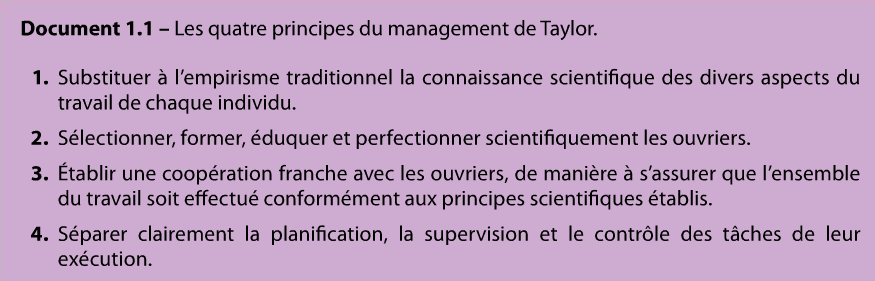
\includegraphics[scale=0.75]{Images/Taylor}
				\end{figure}\noindent
				\point \myul{Avantages}: Cr\'eation de richesse. Entreprises tayloriennes existent encore
				aujourd'hui.\\
				\point \myul{D\'esavantages}: Le travaille \`a la chaine et en masse d\'evalorise le travail 
				de l'ouvrier (ne se rend pas compte de l'utilit\'e de son travail) $\rightarrow$ 
				d\'emotivation et manque d'attention $\rightarrow$ risque d'accidents/blessures.
			\paragraph{Henry Ford}~\\
				\point \hl{Chaine de production} qui r\'eduit les d\'eplacements des travailleurs. \\
					\alinea \hl{Transformation de l'ouvrier en consommateur} en le payant plus 
					$\rightarrow$ cr\'eation d'une classe \\
					\alinea moyenne.
			\paragraph{Frank et Lillian Gilbreth}~\\
				\point Suppression des \hl{mouvement inutiles} des ouvriers\\
				\point \myul{Therblings}: \red{Syst\`eme de classification des mouvements invent\'e par les
					Gilbreth r\'epertoriant \\
					\alinea 17 gestes \'el\'ementaires de la main}
			\paragraph{Henry Gantt}~\\
				\point \hl{Prime aux ouvriers} si le travail est fait dans les temps, prime au
				contremaître et prime\\
				\alinea d'\'equipe.
		\subsubsection{La th\'eorie administrative g\'en\'erale}
			\point \myul{Acteurs Principaux} : Henry Fayol, Max Weber.\\
			\point Se base sur l'organisation globale de l'entreprise pour la rendre plus efficace.
			\paragraph{Henry Fayol}~\\
				\point Organisation autour du \hl{travail des dirigeants}, des managers.\\
				\point \myul{POCCC}: \hl{Planifier, Organiser, Commander, Coordonner, Contr\^oler}.\\
				\point Plus \hl{humaniste} que Taylor, permet \hl{l'initiative} chez les ouvriers.
				\vfill
				\begin{figure}[H]
					\centering
					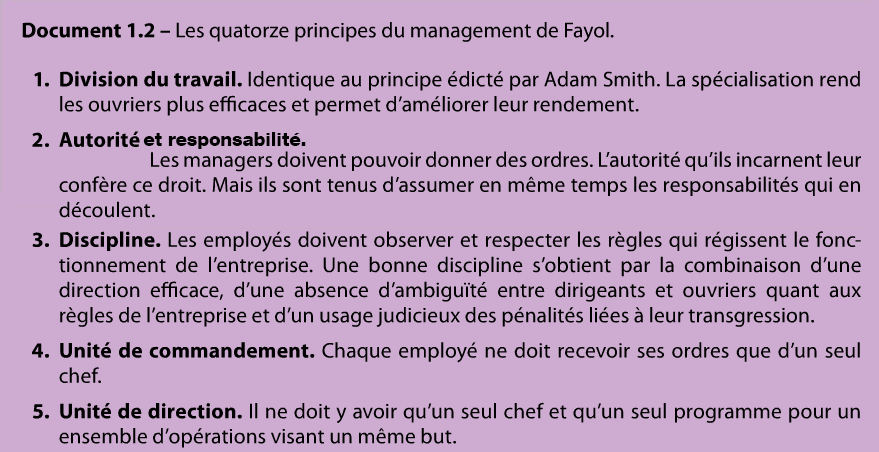
\includegraphics[scale=0.75]{Images/Fayol0}
				\end{figure}
				\begin{figure}[H]
					\centering
					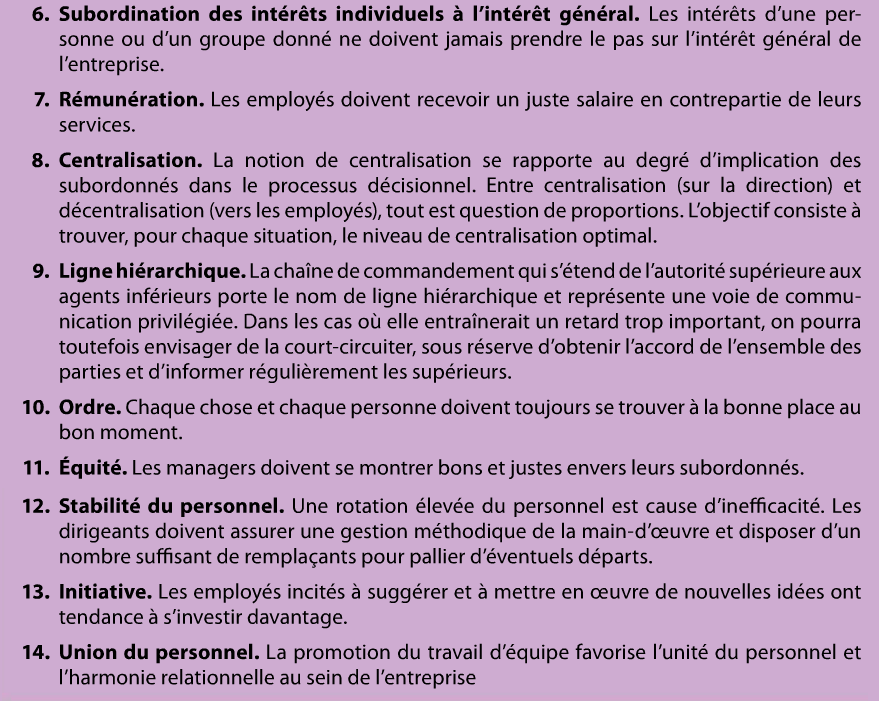
\includegraphics[scale=0.75]{Images/Fayol1}
				\end{figure}
			\paragraph{Max Weber}~\\
				\point Imagine un organisation th\'eoriquement id\'eale : la \myul{bureaucratie}.\\
				\point Travail \hl{d\'eshumanis\'e et \'equitable}. Tout est standardis\'e : Question A 
					= R\'eponse 56, ... On ne\\ 
					\alinea demande pas de r\'efl\'echir, juste d'appliquer des r\`egles \'etablies.\\
				\point \myul{Avantages} : Peu co\^uteux et fait gagner beaucoup de temps.\\
				\point \myul{D\'esavantages} : Impossible de \\
					\alinea pr\'evoir toutes les demandes $\rightarrow$ limit\'e en puissance.
				\begin{figure}[H]
					\centering
					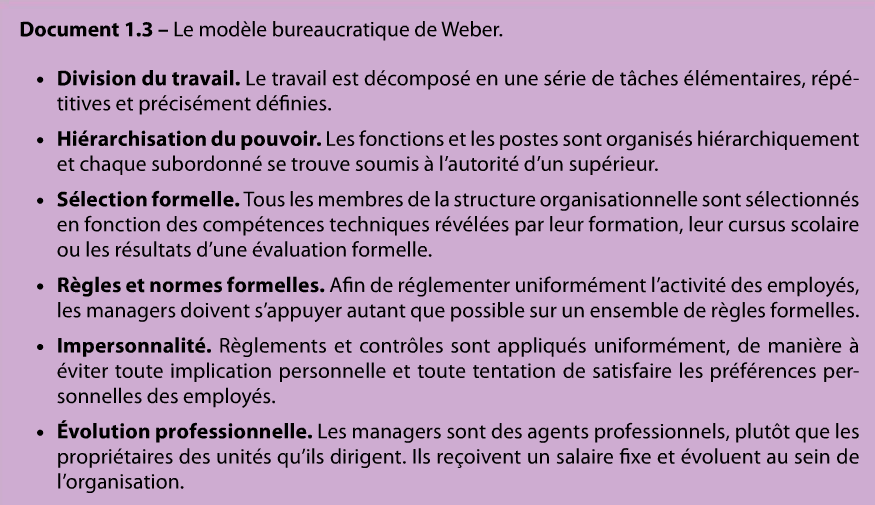
\includegraphics[scale=0.75]{Images/Weber}
				\end{figure}
	\subsection{L'\'ecole des relations humaines}
		\red{Vise \`a stopper la pens\'ee humains=machines. R\'epond aux attentes de l'\'epoque.}
		\subsubsection{Les humanitaires}
			\point \myul{Robert Owen} : R\`eglementation sur les \hl{horaires} de travail, 
				sur le travail des enfants. \\
				\alinea \hl{Reproche que les machines soient mieux trait\'ees que les 
				ouvriers}. Il veut am\'eliorer les \\
				\alinea \hl{conditions de travail} des ouvriers pour augmenter
				la productivit\'e.\\
			\point \myul{Hugo Munsterberg} : Premier \`a faire un lien entre \'ecole classique et \'ecole
				des relations\\
				\alinea humaines. Il \'etudie les individus et introduit les tests psychologiques \`a 
				l'embauche.\\
			\point \myul{Mary Parker Follett} : Les managers et les employ\'es doivent se consid\'erer comme
				partenaire.\\
				\alinea L'int\'erêt de l'individu ne doit pas s'effacer devant celui du groupe 
				\hl{(contraire de Fayol)}.\\
			\point \myul{Chester Barnard} : La r\'eussite d\'epend de la coop\'eration et de la soumission \`a
				l'autorit\'e \\
				\alinea des employ\'es. Mais aussi de la relation de l'entreprise avec ses 
				\hl{intervenant externes}.\\
			\point \myul{Elton Mayo} : \'Etudes sur l'ergonomie de travail. Les lieux n'influencent
				pas la productivit\'e\\
				\alinea mais une \hl{dynamique positive de groupe} oui. Est \`a la base de l'appellation 
				\hl{"effet d'Hawthorne"}\\
				\alinea qui d\'esigne le lien comportement/sentiment et l'importance du poids du groupe
				sur les\\ 
				\alinea comportements individuels.
		\subsubsection{Satisfaction de l'employ\'e}
			\point \myul{Dale Carnegie} : Manipuler les sentiments des gens permet de r\'eussir au mieux.\\
			\point \myul{Abraham Maslow} : 5 besoins essentiels : physiologiques, s\'ecurit\'e, appartenance,
				estime et\\
				\alinea auto-accomplissement (Chapitre 12).\\
			\point \myul{Douglas McGregor} : Th\'eorie X et Th\'eorie Y (Chapitre 12).
	\subsection{L'\'ecole quantitative}
		\red{Recherche op\'erationnelle, statistique et mod\`ele math\'ematiques d'optimisation
		aident le manager.}
	\subsection{Les th\'eories unificatrices}
		\subsubsection{L'approche par processus de Koontz}
			\point \red{Introduite par Fayol, cette approche se base sur trois principes : planifier,
				organiser et\\
				\alinea commander.}
		\subsubsection{L'approche syst\'emique}
			\point \myul{Syst\`eme} : \red{Tout coh\'erent compos\'e d'\'el\'ements interd\'ependants}\\
			\point Cette approche consid\`ere une entreprise comme un \hl{syst\`eme} complexe et analyse
				ses \\
				\alinea diff\'erentes parties et les \hl{interactions} entre ces parties. Elle reconnaît
				qu'une\\
				\alinea entreprise est un \hl{syst\`eme ouvert} totalement d\'ependant de son
				environnement\\
			\point \myul{Syst\`emes ferm\'es} : \red{syst\`emes qui n'interagissent pas avec leur 
			    environnement et qui\\
				\alinea n'en subissent aucune cons\'equence}\\
			\point \myul{Syst\`emes ouverts} : \red{syst\`emes qui interagissent dynamiquement avec leur 
			    environnement et\\
				\alinea qui transforment les ressources qu'ils traitent}\\
			\point Voici trois approches de parties prenantes, faisant partie de l'environnement; 
				plus on descend\\\alinea et plus l'approche est susceptible  d'être consid\'er\'ee 
				comme \'ethique.
			\begin{itemize}
			\setlength{\itemsep}{0pt}
			\setlength{\parskip}{0pt}
			\setlength{\parsep}{0pt}
			\item \myul{Approche Shareholder} : \red{Actionnaire conscient des risques, dernier \`a
				être rembours\'e en cas de faillite, mais tout b\'en\'efice (apr\`es salaire, ...)
				lui revient.}
			\item \myul{Approche Stakeholder sens strict} : \red{Le b\'en\'efice revient \`a tous ceux 
				qui y ont particip\'e, y comprit les actionnaires.}
			\item \myul{Approche Stakeholder sens large} : \red{Le b\'en\'efice revient \`a tous ceux qui 
				y ont  particip\'e mais aussi \`a tous ceux affect\'es par la cr\'eation de ce b\'en\'efice.}
			\end{itemize}
			\begin{figure}[H]
				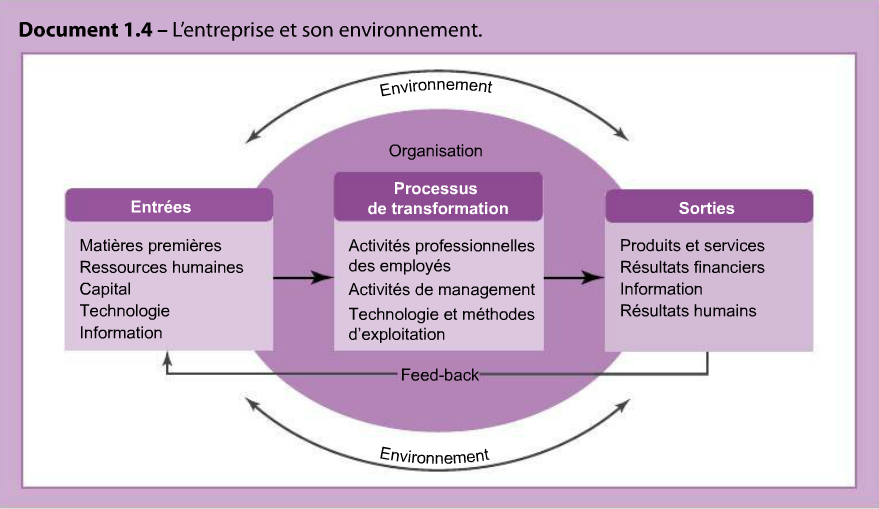
\includegraphics[scale=0.75]{Images/Systeme1}
			\end{figure}
		\subsubsection{Th\'eorie de la contingence}
			\point \red{Pas de m\'ethode universelle, que des approches qui d\'ependent de la situation.
				Et ceci\\
				\alinea selon \hl{quatre variables}:}
				\begin{itemize}
					\setlength{\itemsep}{0pt}
				    \setlength{\parskip}{0pt}
				    \setlength{\parsep}{0pt}
					\item \myul{Taille de l'entreprise} : Plus elle est grande, plus elle est dfficile \`a 
						coordonner.
					\item \myul{Qualification des technologies} : L'organisation de l'entreprise d\'epend 
						de la technologie utilis\'ee en son sein (processus de d\'eveloppement, ...)
					\item \myul{Incertitude environnementale} : La situation d\'epend de l'environnement de 
						l'entreprise et de sa stabilit\'e.
					\item \myul{Particularit\'es individuelles} : La situation d\'epend de l'individu et de 
						ses ambitions, autonomie, capacit\'e \`a tol\'erer l'ambigu\"it\'e, ...
				\end{itemize}
\pagebreak
\section{Chapitre 2: Les m\'etiers du manager}
	\subsection{Qu'est-ce que le management ?}
		\point \myul{Organisation} : Ensemble de personnes rassembl\'ees afin d'atteindre des \hl{objectifs}, 
			par une
			\\\hspace*{0.2cm}\hl{division du travail} et des \hl{fonctions}, grâce \`a des modalit\'es de 
			coordination d\'efinies\\
		\point \myul{Managers} : personnes coordonnant et dirigeant dans une organisation les activit\'es des 
			\\\alinea autres, soit en mode \hl{hi\'erarchique}, soit en mode \hl{transversal}.\\
		\point \myul{Employ\'es} : personnes s'occupant d'une tâche donn\'ee et n'ayant aucune 
			responsabilit\'e \\\alinea de supervision du travail des autres.\\
		\point Il existe \hl{quatre types} de managers : 
			\begin{figure}[H]
				\centering
				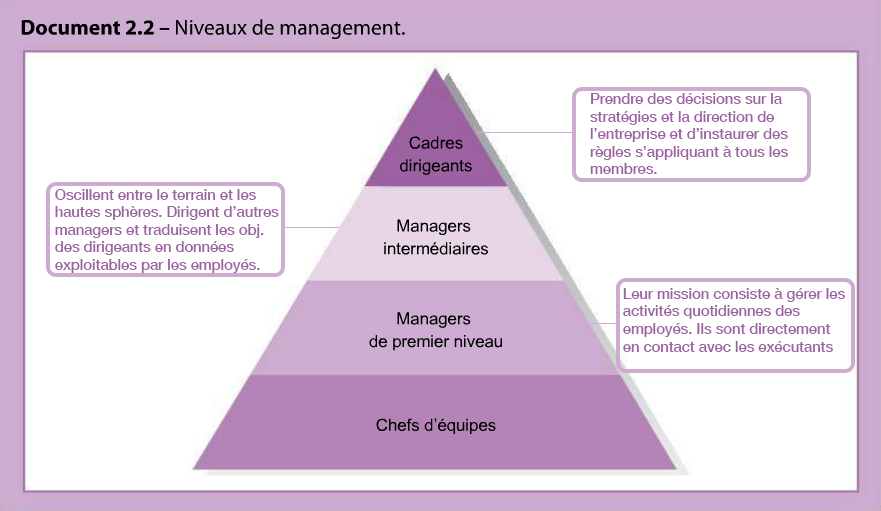
\includegraphics[scale=0.75]{Images/Managers}
			\end{figure}\noindent
		\point \myul{Management} : \red{Processus par lequel des r\'esultats sont obtenus de façon
		    \hl{efficace} 
			\\\alinea et \hl{efficiente}, via et avec la coop\'eration d'autrui.}\\
		\point \myul{Efficacit\'e} : \red{Mesure se r\'ef\'erant au fait d'\hl{atteindre des objectifs}.}
			\\\alinea Pour une firme commerciale, la première condition d'efficacité est la \hl{valorisation}
			par les clients. \\\alinea (Faire en sorte que les clients valorisent les produits de la
			firme).\\
		\point \myul{Efficience} : \red{Mesure se r\'ef\'erant au fait d'effectuer une tâche correctement en
			\\\alinea \hl{minimisant le co\^ut du processus}.} Une \hl{chute du profit} est signe d'un
			\hl{manque}	d'efficience.
		\point \hl{En ne se focalisant que sur l'efficience, on risque de perdre en efficacit\'e.}
	\subsection{Que font les managers ?}
		\point Sur les cinq points que Fayol \'enonçait, on en retient quatre :
		\begin{figure}[H]
			\centering
			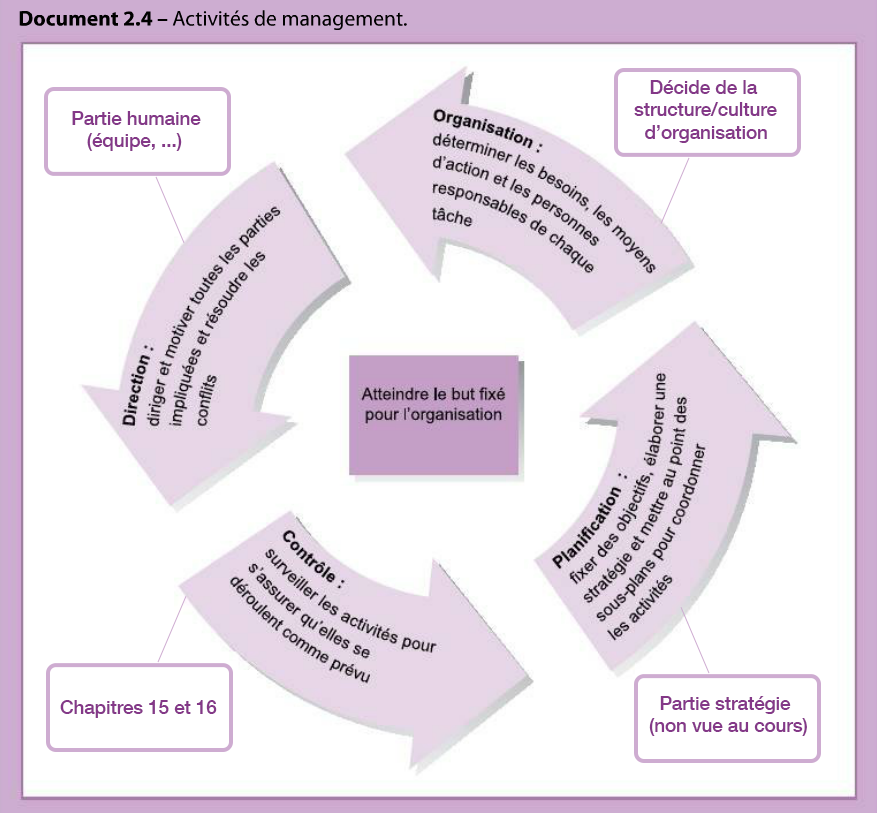
\includegraphics[scale=0.75]{Images/Managers2}
		\end{figure}
		\point \myul{Henri Mintzberg} d\'efinit 10 r\^oles essentiels que doivent assurer les managers:
		\newgeometry{top = 2cm, left = 2cm, right = 2cm, bottom=1.2cm}
		\begin{figure}[H]
			\centering
			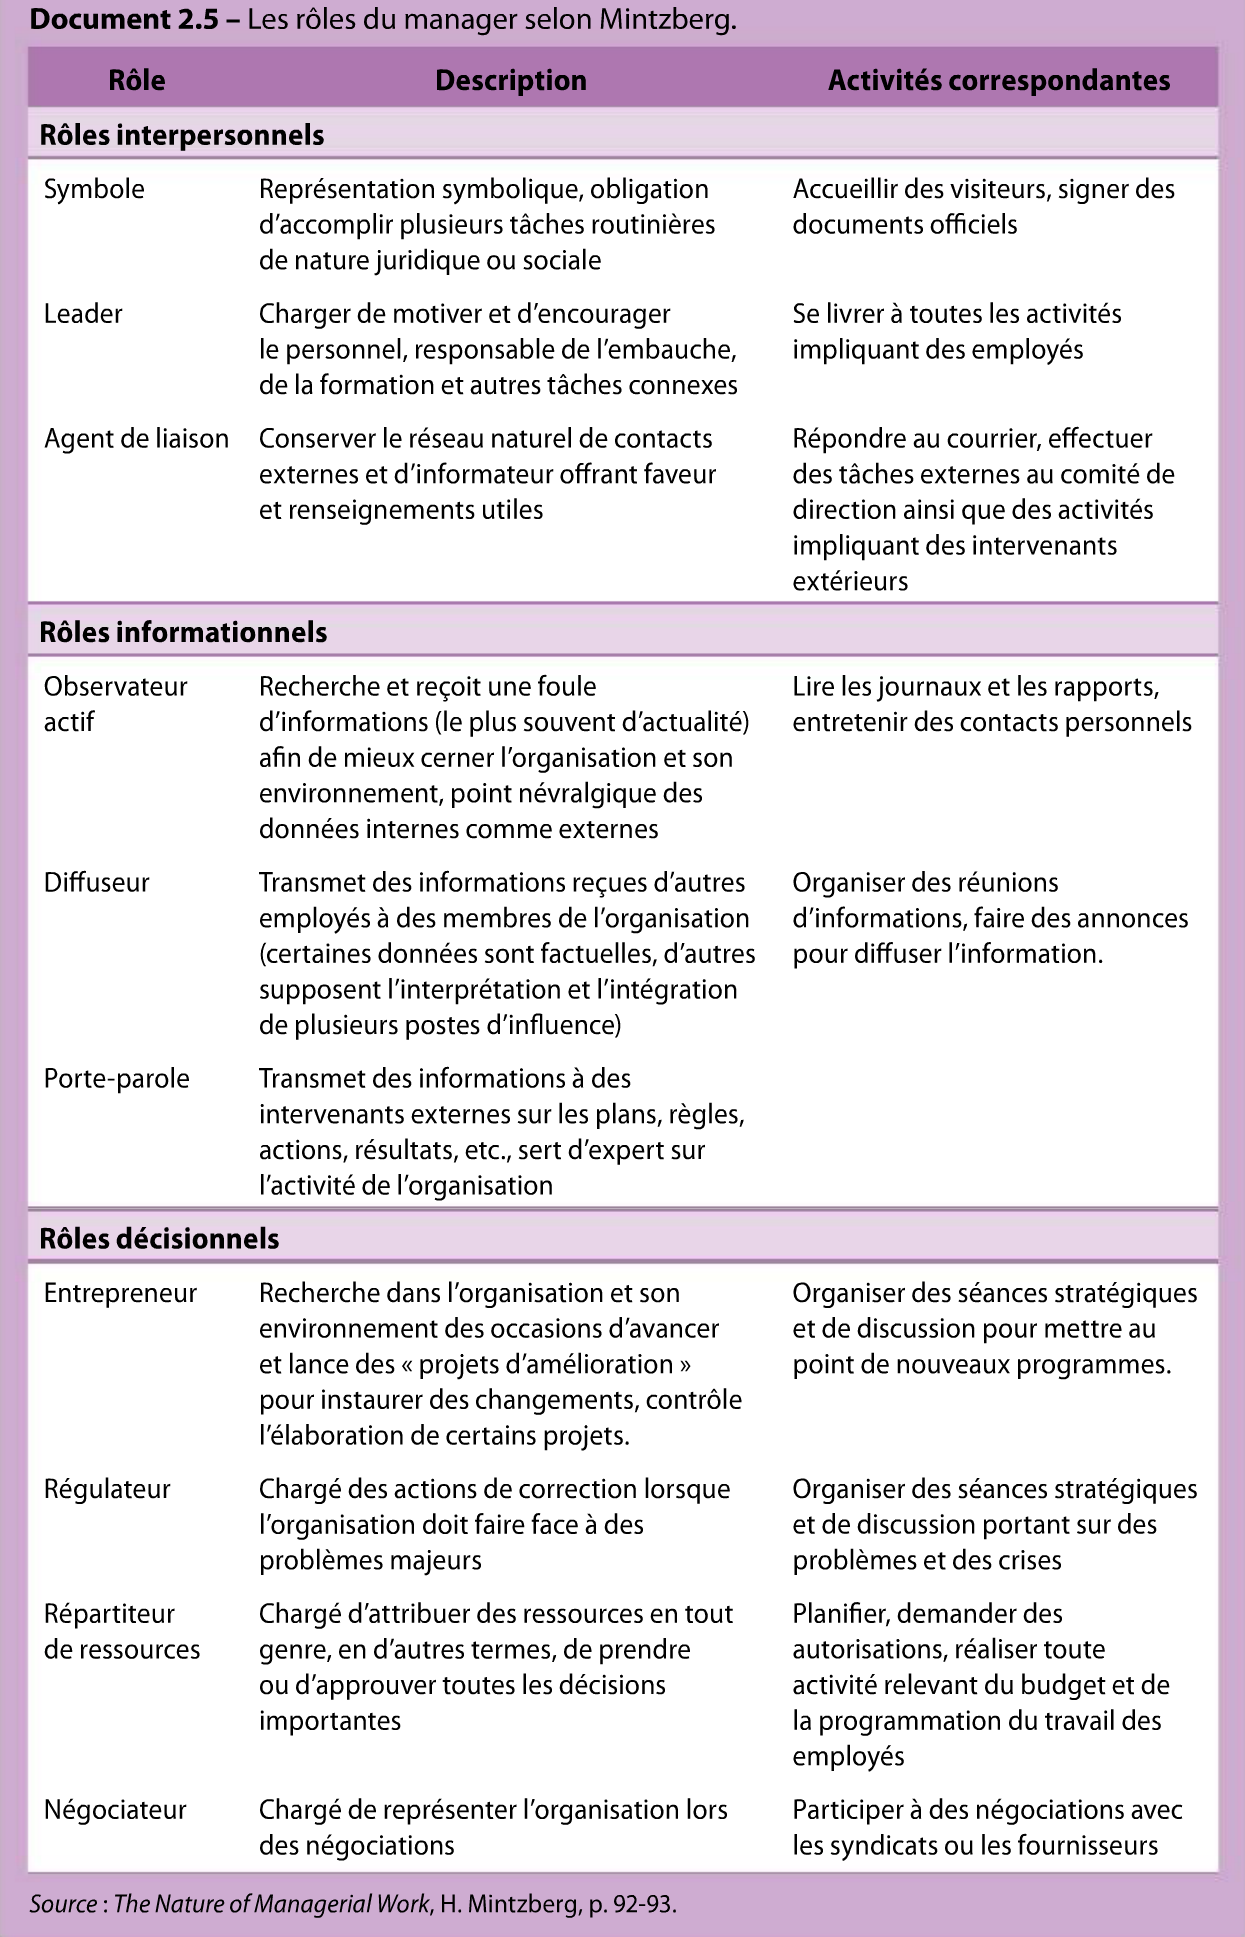
\includegraphics[scale=0.48]{Images/Roles}
		\end{figure}
		\pagebreak\noindent
		\newgeometry{top = 2.5cm, left = 2cm, right = 2cm, bottom=2cm}\noindent
		%
		\paragraph{Manager : un m\'etier universel} ~\\
			\point \myul{Place hi\'erarchique} : Les quatre principes de Fayol restent les même pour un cadre
				ou pour \\
				\alinea un chef d'\'equipe. Plus on est haut dans la pyramide, plus le c\^ot\'e
				\hl{Organisation} sera \\
				\alinea important et moins le cot\'e \hl{Direction} le sera. \\
			\point \myul{ASBL ou autre} : Quel que soit le but, les r\^oles des managers ne change pas\\
			\point \myul{Taille de l'entreprise} : Le r\^ole d'un manager dans une PME est plut\^ot 
				g\'en\'eraliste, \hl{polyvalent}.\\
				\alinea Tandis que celui d'un manager d'une grande entreprise est plus cibl\'e.\\
			\point \myul{Aspects g\'eographiques et culturels} : Le manager doit faire attention aux
				\hl{particularit\'es}\\
				\alinea \hl{culturelles} de son environnement.
\pagebreak
\section{Chapitre 3 : L'environnement du manager}
	\subsection{Vocabulaire}
		\point \myul{Assets stripping} : \red{On se débarrasse de \hl{ce qui n'est pas utile/rentable} et
			qui a de \\\alinea la \hl{valeur}.}\\
		\point \myul{Downsizing} : \red{Diminuer la taille en ne \hl{gardant que les parties les plus
			performantes},\\\alinea les plus rentables et surtout les \hl{mieux valoris\'ees sur le march\'e}
			financier \\\alinea \hl{sans pour autant mettre en p\'eril le core business}.
			Peut aussi conduire à supprimer des \\\alinea activités rentables ne faisant pas partie}
			du core business.
			\\\alinea Peut se faire en faisant de l'assets stripping.\\
		\point \myul{Fond de pension} : \red{Retir\'e du salaire pour ensuite être investit par milliards en 
			bourses.}\\
		\point \myul{SICAV} : \red{Veut investir (avec risque) mais n'a que quelques milliers $\rightarrow$
			fond commun \\\alinea de placement, confi\'e \`a des professionnels qui prennent un pourcentage.}
			\\
		\point \myul{Flux tendu} : \red{C'est le \hl{consommateur} qui met en route la chaîne de 
			production.}\\
		\point \myul{Flux pouss\'e} : \red{Ce sont les \hl{pr\'evisions de vente} qui font produire.}\\
		\point \myul{Just In TIme} : \red{Mani\`ere de se faire livrer des mati\`eres premi\`eres \hl{au 
			moment o\`u on veut}\\\alinea \hl{les transformer en produit fini}}\\
		\point \myul{Outsourcing} : \red{Si c'est plus cher de produire un mat\'eriau que de \hl{l'acheter 
			chez un} \\\alinea \hl{fournisseur}, on va s'externaliser. $/!\setminus$ Si on a jamais 
			pens\'e \`a	produire le mat\'eriau, ce n'est pas \\\alinea de l'outsourcing.}\\
		\point \myul{Kanban} : \red{Gestion des stocks tel que la production de mat\'eriau du processus A pour
			\\\alinea un processus B ne d\'epasse jamais les besoins du processus B.} \\
		\point \myul{Kaizen} : \red{Philosophie d'am\'elioration continue. Libert\'e laiss\'ee aux employ\'es
			afin que \\\alinea ceux ci puissent am\'eliorer leur environnement de travail pour être plus
			productifs.}
	\subsection{Monde moderne}
		\subsubsection{Changement technologique}
			De nos jours, l'enti\`eret\'e du monde se trouve en concurrence sur tous les march\'es. Les
			entreprises ne partent plus du b\'en\'efice qu'elle souhaite mais de ce que le
			client est prêt \`a payer.\red{\hl{$\rightarrow$ Avec la technologie, on a invers\'e le
			rapport de 	force entre le fournisseur et le client}}.
		\subsubsection{Changement sur les march\'es financiers}
			\alinea Avant, on investissait dans le local parce que les march\'es/bourses \'etrangers 
				\'etaient inaccessibles. Maintenant que l'on peut investir partout, \hl{ce sont les 
				investisseurs} \red{\hl{et les financiers, qui mettent la pression}} et les 
				entreprises qui sont moins  rentables que la moyenne du secteur sont d\'elaiss\'ees/ 
				ferm\'ees afin de faire remonter sa moyenne aupr\`es des actionnaires.\\
			\alinea Ce qui implique que maintenant on ne cherche \hl{plus seulement \`a \^etre 
				rentable, mais \`a \^etre le plus rentable. Ce qui tend \`a privil\'egier les 
				strat\'egies \`a court terme}.
		\subsubsection{Le management japonais}
			\point \myul{Logique soustractive} : Avant, on rajoutait au prix de vente pour gonfler le 
				b\'en\'efice.\\\alinea Maintenant, on minimise les co\^uts pour gonfler le b\'en\'efice.\\
			\point Travail en \hl{flux tendu}, avec stock \hl{Just In Time} et \hl{Kanban}.\\
			\point Mentalit\'e \hl{Kaizen} d'am\'elioration continue, prendre ailleurs les id\'ees qui
				marchent  
				le mieux \\\alinea pour les int\'egrer \`a son entreprise et motiver les employ\'es \`a
				s'am\'eliorer constamment.\\
			\point \hl{Outsourcing} et \hl{qualit\'e totale} impliquant la responsabilisation
				des employés \\\alinea (arrêt de la chaîne de production d\'es qu'un  
				d\'efaut est d\'etect\'e.
	\subsection{Incertitude environnementale}
		\begin{figure}[H]
			\centering
			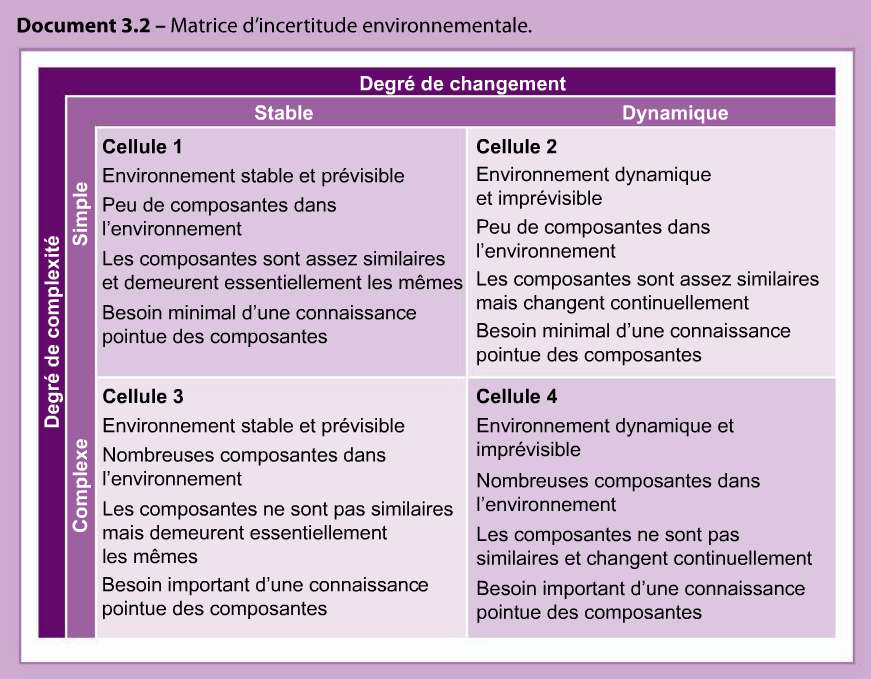
\includegraphics[scale=0.7]{Images/environnement0}
		\end{figure}
		\point On parle d'\myul{environnement dynamique} s'il \hl{change souvent} et d'\myul{environnement 
			stable} si la \\\alinea fr\'equence de changement est faible. (pas de concurrent, pas de perc\'ee 
			technologique, ...).\\
		\point On parle d'\myul{environnement complexe} dans le cas o\`u il y a \hl{beaucoup de composantes}  
			dans \\\alinea l'environnement et si l'organisation doit avoir un niveau de connaissance 
			relativement \'elev\'e\\\alinea envers elles.\\
		\point Plus l'environnement est complexe et dynamique plus il est \hl{difficile de prendre les 
			bonnes \\\alinea d\'ecisions}.\\
		\point \hl{Avoir de bonnes relations avec les parties prenantes} de l'organisation permet 
			d'avoir \\\alinea une information compl\`ete sur son environnement. 
			\\\alinea \red{$\rightarrow$Plus les relations sont solides, plus les managers auront un impact 
			sur les r\'esultats de\\\alinea l'organisation}.
		\begin{figure}[H]
			\centering
			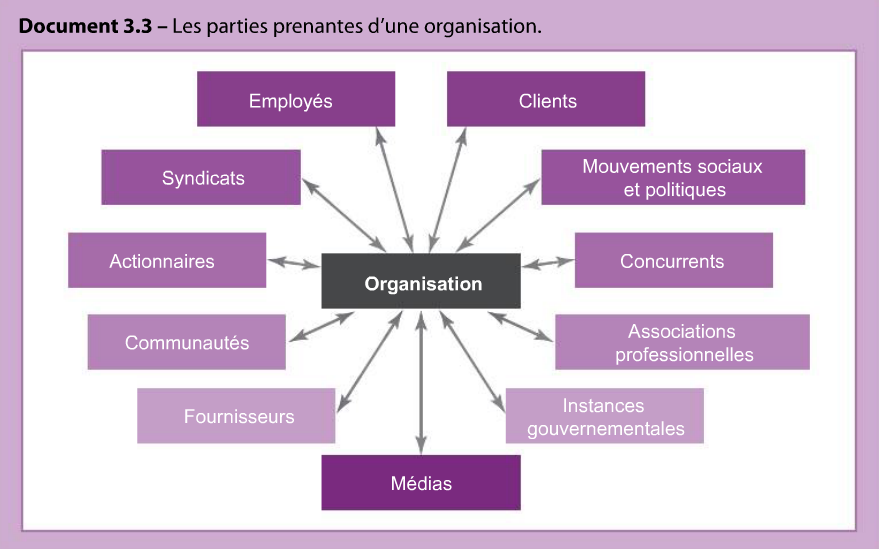
\includegraphics[scale=0.75]{Images/environnement1}
		\end{figure}
	\subsection{Mondialisation}
		\point \myul{Firme locale} : Exporte un peu mais principalement \hl{local}.\\
		\point \myul{Multinationale} : \hl{Un si\`ege social local important} et beaucoup d'usines dans le
			monde.\\
		\point \myul{Firme globale} : Beaucoup de si\`eges/d'usines importantes r\'eparties dans le monde.
			\\\alinea \hl{Pas de QG}.\\ 
		\point \myul{Firme internationale} : Mode de fonctionnement et prise de d\'ecision 
			\hl{propre \`a chaque pays}
			\\\alinea Engage des personnes sp\'ecifiques \`a la r\'egion, adapt\'ees \`a la culture locale.\\
		\point \hl{Les raisons de devenir multinational} : \hl{la r\'epartition des risques}, 
			\hl{la proximit\'e} \\\alinea des clients ou des ressources et les \hl{avantages 
			comparatifs} (taxes, ...). \\
		\point \myul{Licence} : Permis d'utiliser une marque ou une recette \`a des fins commerciales.\\
		\point \myul{Franchise} : Ensemble de biens (restaurants, ...) assign\'es \`a une marque (McDo, ...).				\\
		\point \myul{Alliance strat\'egique internationale} : Partenariat visant le \hl{partage des 
			ressources} et \\\alinea de connaissances avec des partenaires internationaux.\\
		\point \myul{Joint-Venture} : Forme particuli\`ere d'alliance strat\'egique qui implique 
			\hl{la cr\'eation } \\\alinea \hl{d'une nouvelle entit\'e ind\'ependante} et dont les
			 partenaires partagent la propri\'et\'e.\\
			\begin{figure}[H]
				\centering
				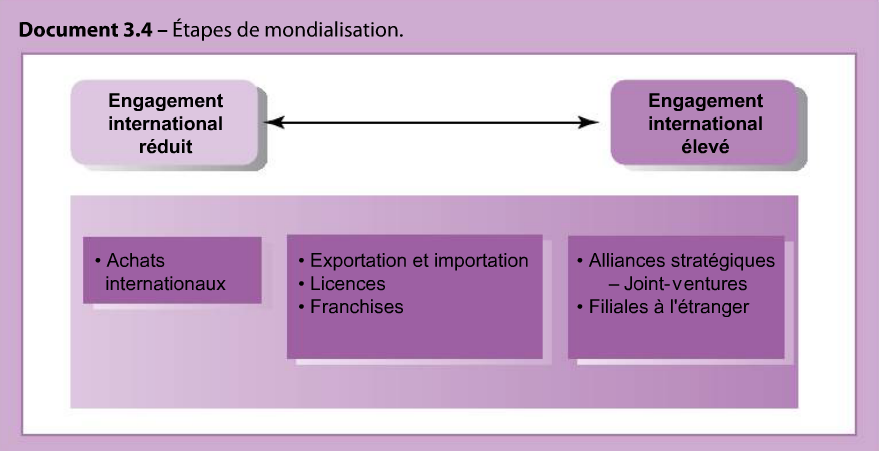
\includegraphics[scale=0.5]{Images/mondialisation}
			\end{figure}
	\subsection{La soci\'et\'e et les Organisations}
		\begin{figure}[H]
			\centering
			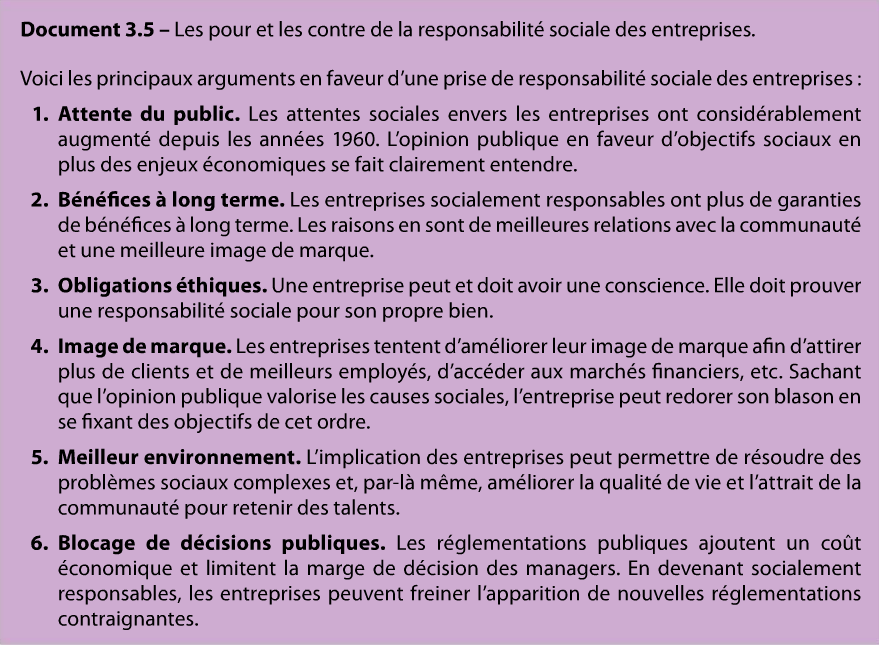
\includegraphics[scale=0.725]{Images/societeplus1}
		\end{figure}
		\begin{figure}[H]
			\centering
			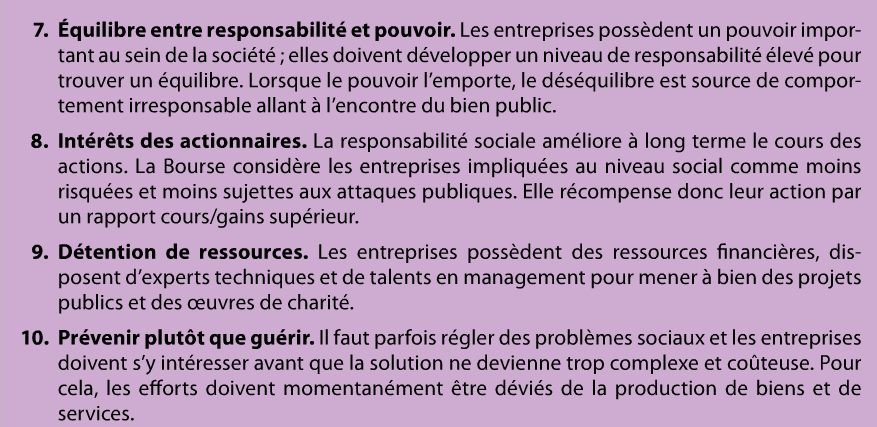
\includegraphics[scale=0.725]{Images/societeplus2}
		\end{figure}\noindent
		\begin{figure}[H]
			\centering
			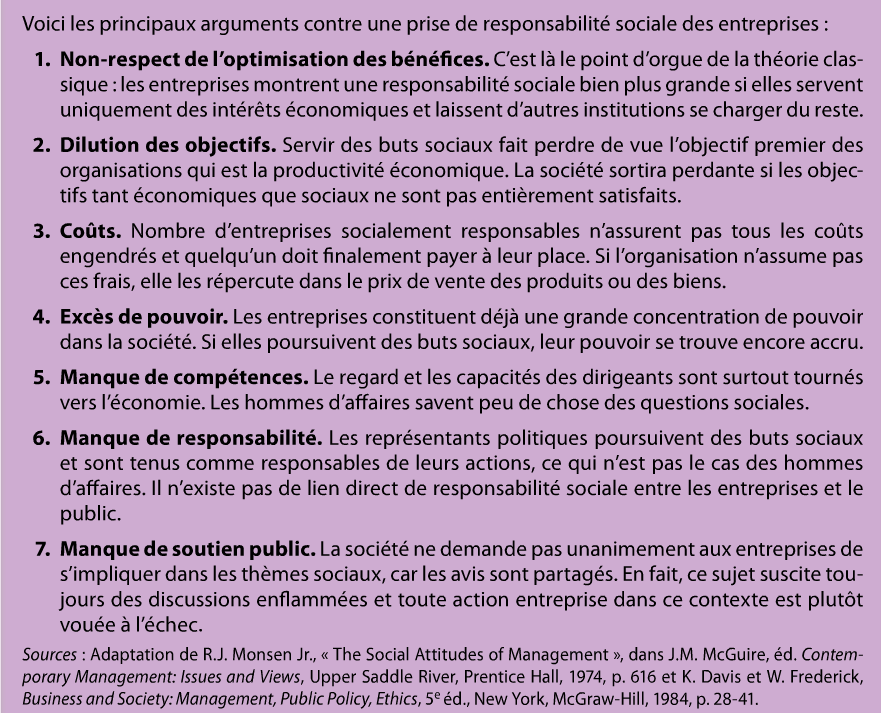
\includegraphics[scale=0.725]{Images/societemoins}
		\end{figure}\noindent
		\point \myul{Obligation sociale} : Remplir ses responsabilit\'es\hl{ \'economiques et juridiques}.\\
		\point \myul{Sensibilit\'e sociale} : Dissocier ce qui est \hl{bien et mal envers la soci\'et\'e} et  
		ne garder \\\alinea que le bien.
		\subsubsection{Durabilit\'e}
			\red{La durabilit\'e est la capacit\'e d'une organisation \`a atteindre ses objectifs et \`a
			augmenter
			sa valeur actionnariale \`a long terme en int\'egrant des \hl{opportunit\'es \'economiques,
			environnementales et} \hl{sociales \`a sa strat\'egie commerciale}.}
		\subsubsection{Programme \'ethique complet}
			\point \myul{Code d'\'ethique} : Base pour un programme s'il est pris au s\'erieux.
				\begin{itemize}
					\setlength{\itemsep}{0pt}
				    \setlength{\parskip}{0pt}
				    \setlength{\parsep}{0pt}
				    \item \hl{R\'eduire les ambigu\"it\'es} sur ce qui est bon ou non.
				    \item \^Etre assez pr\'ecis dans les r\`egles mais laisser une \hl{libert\'e de jugement} 	
				    	possible.
				    \item Impliquer les hauts plac\'es \`a suivre le code.
				\end{itemize}
			\point \myul{Leadership \'ethique} : Le manager r\'epond aux crit\`eres suivants:
				\begin{itemize}
					\setlength{\itemsep}{0pt}
				    \setlength{\parskip}{0pt}
				    \setlength{\parsep}{0pt}
				    \item Montrer l'exemple.
				    \item \hl{Punir ou r\'ecompenser publiquement} les employ\'es selon leur comportement.
				\end{itemize}
			\point \myul{Formations \`a l'\'ethique} : Formations \hl{cibl\'ees} au vu des probl\`emes
				rencontr\'es.\\
			\point \myul{Entretiens d'embauche} : Embaucher uniquement des personnes correspondant aux
				\\\alinea valeurs \'ethiques de l'organisation
	\subsection{Main d'oeuvre}
		\point \myul{Baby boomers} : N\'es entre 46 et 64, majorit\'e de la main d'oeuvre actuelle.\\
		\point \myul{G\'en\'eration X} : N\'ee entre 65 et 77, peu nombreux.\\
		\point \myul{G\'en\'eration Y} : N\'ee entre 78 et 94, impactent l'environnement par la technologie,
			\\\alinea leurs style vestimentaire, ... Donnent beaucoup d'importance \`a leur vie de famille
			\\\alinea \red{$\rightarrow$ Proposer des r\'eductions et offres sur des \hl{activit\'es 
			familiales.}}\\
		\point \myul{G\'en\'eration Z} : Adolescents actuels, ont toujours connu la technologie qui 
			\\\alinea personnalise tout en fonction de l'individu.\\
		\point \hl{Savoir \`a quelle g\'en\'eration on a affaire permet de mieux comprendre et de mieux 
			g\'erer}
			\\\alinea \hl{le personnel.}\\
		\point \myul{Emplois atypiques} : Les consultants, les mi-temps, ... Peuvent ne pas s'identifier 
			\\\alinea comme membre \`a part enti\`ere de l'organisation. Trouver des techniques pour les 
			\\\alinea \hl{faire sentir "comme chez eux".}
		\begin{figure}[H]
			\centering
			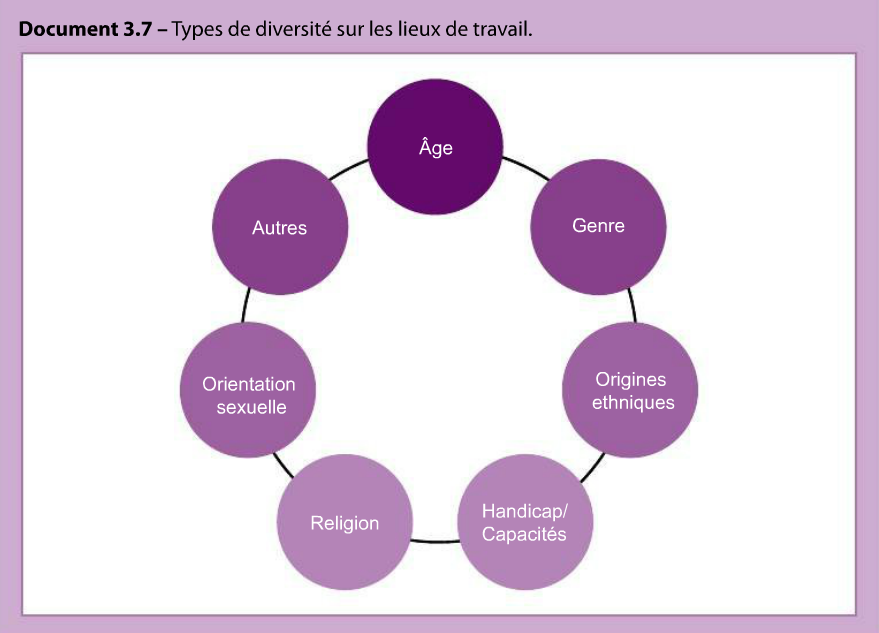
\includegraphics[scale=0.75]{Images/diversite}
		\end{figure}
\section{Chapitre 4 : La prise de d\'ecision}
	\subsection{Le processus d\'ecisionnel}
		\begin{figure}[H]
			\centering
			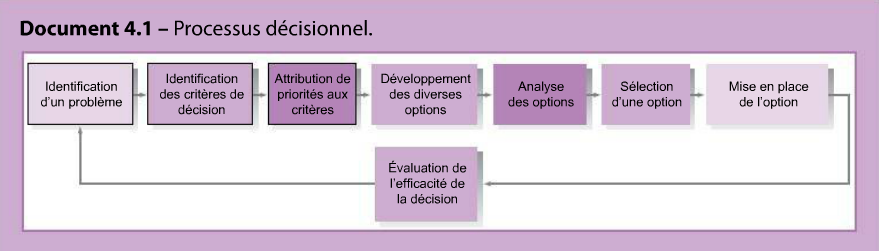
\includegraphics[scale=0.75]{Images/decision1}
		\end{figure}
		\pagebreak\noindent
		\begin{itemize}
			\setlength{\itemsep}{0pt}
		    \setlength{\parskip}{0pt}
		    \setlength{\parsep}{0pt}
			\item \myul{\'Etape 1: l'identification d'un probl\`eme} :
				\red{\hl{Comparer la situation actuelle}} avec une situation normale, et identifier
				ce qui ne va pas.
			\item \myul{\'Etape 2: l'identification des crit\`eres de d\'ecision} : 
				Identifier les \red{\hl{aspects importants}} pour la prise de d\'ecision.
			\item \myul{\'Etape 3: l'attribution d'une pond\'eration aux crit\`eres} : 
				Identifier quels aspects choisis \`a l'\'etape 2 sont plus importants que d'autres.
			\item \myul{\'Etape 4: d\'eveloppement des diverses options} : 
				Apporter \red{\hl{plusieurs solutions possible}}, elles ne doivent pas encore être optimales.
			\item \myul{\'Etape 5: analyse des options} : 
				\red{\hl{\'Evaluer}} les solutions de l'\'etape 4 selon la pond\'eration de l'\'etape 3.
			\item \myul{\'Etape 6: s\'election d'une option} : 
				Choisir la solution qui a obtenu\red{\hl{ le meilleur score}} \`a l'\'etape pr\'ec\'edente.
			\item \myul{\'Etape 7: mise en place de l'option} :
				\red{\hl{Mettre en oeuvre}} la solution choisie, cette \'etape peut encore \'eventuellement
				 \'echouer. 
			\item \myul{\'Etape 8: \'evaluation de l'efficacit\'e de la solution} : 
				D\'ecider si la \red{\hl{solution choisie \'etait la bonne}} (afin de r\'eajuster le
				processus pour la prochaine fois.
		\end{itemize}
		\begin{figure}[H]
			\centering
			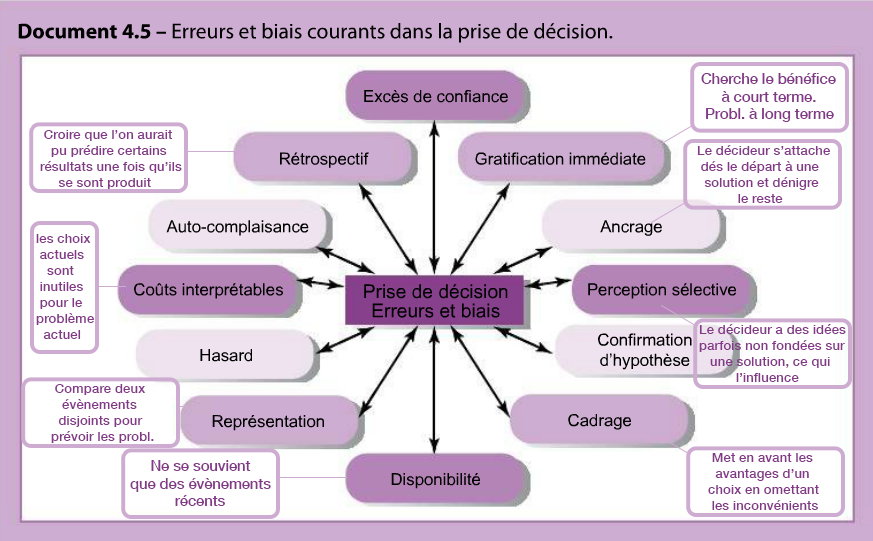
\includegraphics[scale=0.75]{Images/erreurs}
		\end{figure}
		\begin{figure}[H]
			\centering
			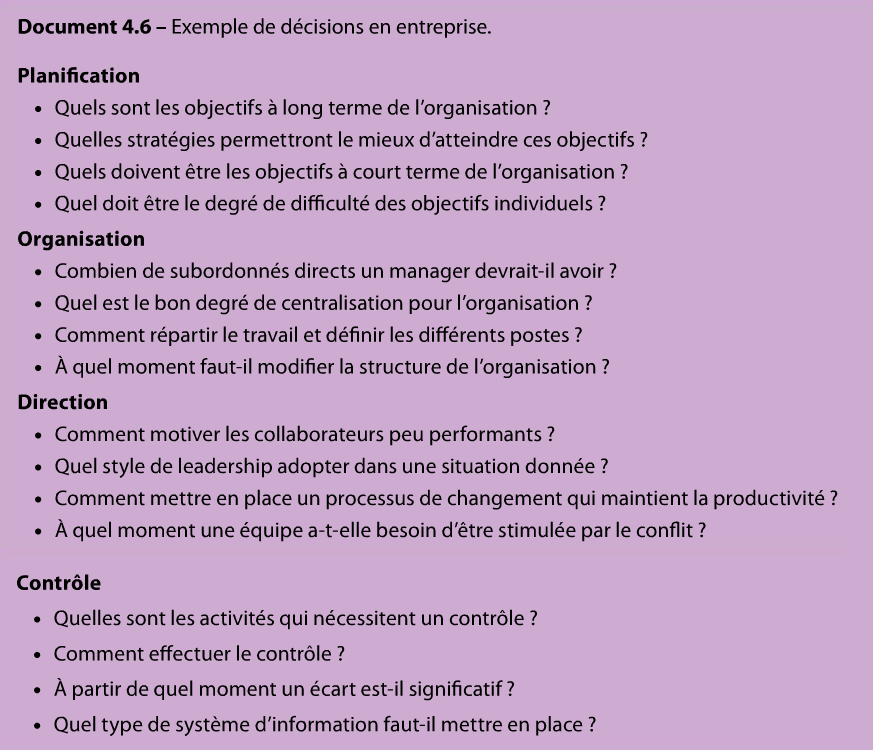
\includegraphics[scale=0.75]{Images/decision2}
		\end{figure}
	\subsection{Les trois approches de la prise de d\'ecision}
		\subsubsection{Le mod\`ele rationnel}
			\point \red{Se dit d'une d\'ecision coh\'erente et maximisant l'utilit\'e dans la limite des
				contraintes donn\'ees}\\
			\point \hl{Irr\'ealisable en pratique car personne n'est omniscient}.
		\subsubsection{La rationalit\'e limit\'ee}
			\point \red{Prise de d\'ecision rationnelle limit\'ee par la capacit\'e de gestion d'information.}
				\\
				\alinea \hl{On accepte une solution en acceptant le fait qu'il soit possible qu'elle ne}\\
				\alinea \hl{soit pas optimale}\\
			\point \myul{Choix d'alternative satisfaisante} : Processus de d\'ecision \hl{s'arr\^etant au 
				premier}\\\alinea \hl{choix satisfaisant}.\\
			\point \myul{Escalade d'engagement} : renforcement d'engagement envers une d\'ecision ant\'erieure	
				\\
				\alinea en d\'epit de r\'esultats non satisfaisant (ou d'informations n\'egative).
		\subsubsection{L'intuition}
			\begin{figure}[H]
				\centering
				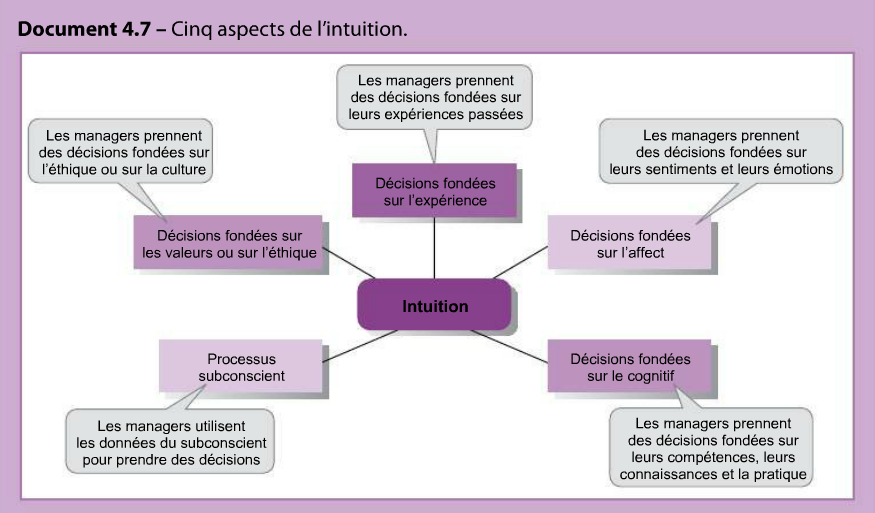
\includegraphics[scale=0.75]{Images/intuition}
			\end{figure}
	\subsection{Types de probl\`eme et contexte de d\'ecision}
		\point \myul{Probl\`emes structur\'es} : \red{probl\`emes connus et simples, familiers et faciles \`a
			cerner}\\
		\point \myul{Probl\`emes non structur\'es} : \red{probl\`emes \`a information ambiguë ou incompl\`ete, 
			\\
			\alinea probl\`eme inhabituel}\\
		\point \myul{D\'ecisions programm\'ees} : \red{D\'ecisions r\'ep\'etitives pouvant être g\'er\'ees par 	
			une approche\\
			\alinea routini\`ere, habituelle.} M\'ethode appliqu\'ee aux probl\`emes structur\'es. 3 
			orientations :
			\begin{itemize}
				\setlength{\itemsep}{0pt}
			    \setlength{\parskip}{0pt}
			    \setlength{\parsep}{0pt}
			    \item \myul{Proc\'edure} : \hl{S\'erie de r\`egles} utilis\'ees pour savoir quelle solution
			    	appliquer.
			    \item \myul{R\`egle} : Affirmation explicite indiquant \hl{ce qu'on doit faire dans une}
			    	\hl{circonstance donn\'ee}
			    \item \myul{Ligne de conduite} : Orientation g\'en\'erale de cadrage pour les d\'ecideurs.\\
			    	\hl{Demande un jugement et une interpr\'etation de la part du d\'ecideur} 
			\end{itemize}
		\point \myul{D\'ecisions non programm\'ees} : \red{d\'ecisions sp\'ecifiques visant \`a \hl{r\'esoudre 
			un probl\`eme} \\\alinea \hl{sp\'ecifique}}\\
		\point \myul{Certitude} : \red{Contexte dans lequel le d\'ecideur \hl{connai\^it le r\'esultat} de 
			chaque option possible}\\
		\point \myul{Risque} : \red{Contexte dans lequel le d\'ecideur peut \hl{estimer la probabilit\'e} de
			certains r\'esultats}\\
		\point \myul{Incertitude} : \red{Contexte dans lequel le d\'ecideur \hl{ne peut ni conna\^itre les
			r\'esultats ni}\\\alinea \hl{estimer les probabilit\'es}} 
		\begin{figure}[H]
			\centering
			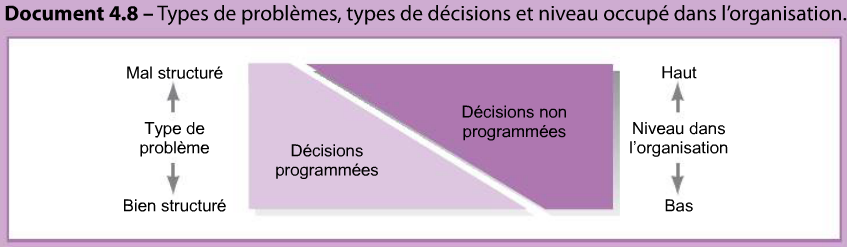
\includegraphics[scale=0.5]{Images/decision3}
		\end{figure}\noindent
	\subsection{D\'ecisions de groupe}
		\begin{figure}[H]
			\centering
			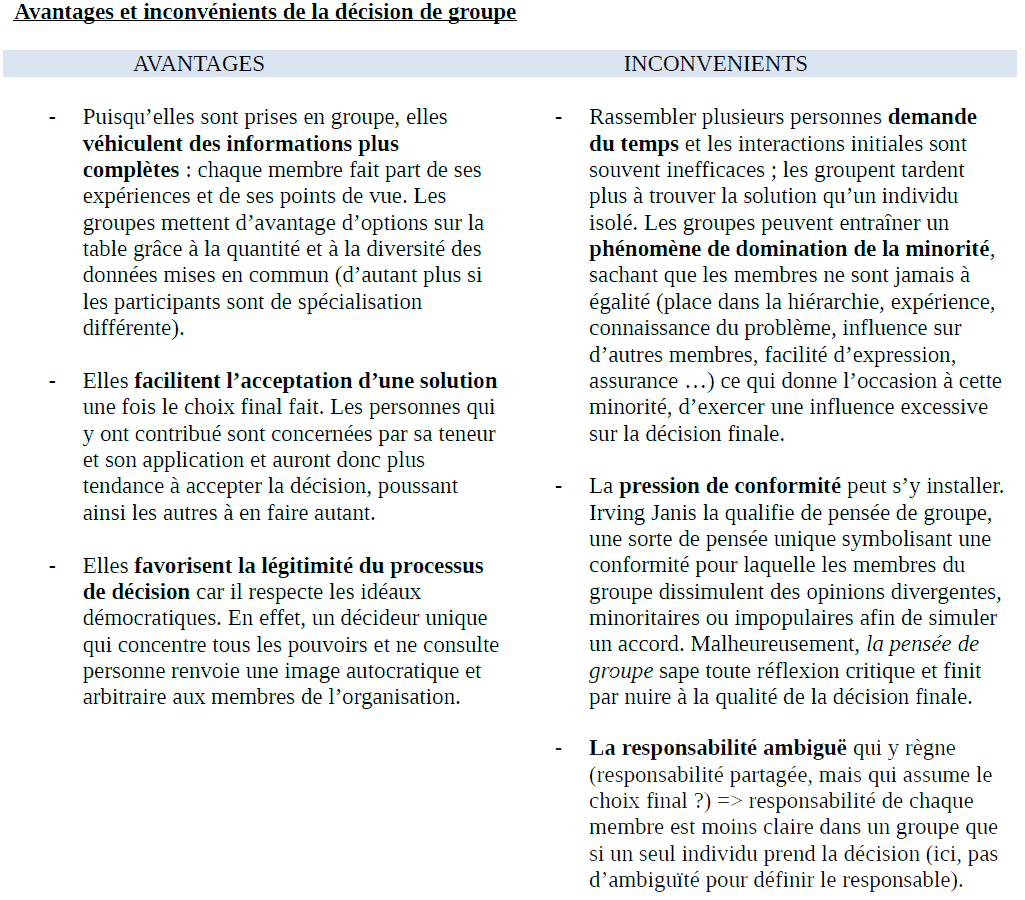
\includegraphics[scale=0.65]{Images/decision_groupe}
		\end{figure}\noindent
		\point \myul{Pens\'ee de groupe} : Tendance d'un groupe \`a \hl{dissimuler des id\'ees divergentes}  
			pour simuler \\\alinea un accord de groupe.\\
		\point \myul{Brainstorming} : R\'eunion permettant de proposer \hl{les id\'ees les plus farfelues} que 
			l'on \\\alinea enregistre avant de les \'evaluer.\\
		\point \myul{Groupe nominal} : Rassemblement d'\hl{id\'ees anonymes} afin qu'une id\'ee ne soit pas 
			attach\'ee \\\alinea \`a une personne.\\
		\point \myul{R\'eunions \'electronique} : Même id\'ee que le groupe nominal où les personnes ne sont
			pas \\\alinea pr\'esentes physiquement.\\
		\point On parle de \myul{d\'ecisions strat\'egiques} pour le long terme et de \myul{d\'ecisions 
			tactiques} pour le \\\alinea court terme, avec lesquelles il est facile de faire marche arri\`ere.
			\\
		\point La culture et la cr\'eativit\'e influencent les prises de d\'ecision en groupe
		\begin{figure}[H]
			\centering
			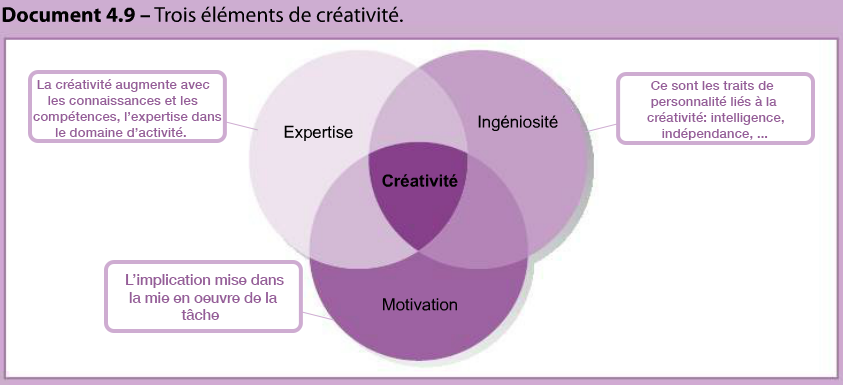
\includegraphics[scale=0.80]{Images/creativite}
		\end{figure}
	\subsection{Outils facilitant la d\'ecision}
		\point \myul{Syst\`emes experts} : \red{Logiciels \hl{agissant comme un expert} pour les probl\`emes 
			non structur\'es.}
		\point \myul{R\'eseaux neuronaux} : \red{Logiciels \hl{imitant le cerveau humain} pour la prise de 
			d\'ecision}
\pagebreak
\section{Chapitre 6: L'entrepreneuriat et les entrepreneurs}
	\point \myul{Entrepreneuriat} : \red{Processus consistant \`a \hl{lancer un projet \`a partir d'une 
		opportunit\'e} \\\alinea d'affaires, \`a organiser les ressources n\'ecessaires et \`a 
		en assumer les risques autant que les\\\alinea b\'en\'efices}
	\begin{figure}[H]
		\centering
		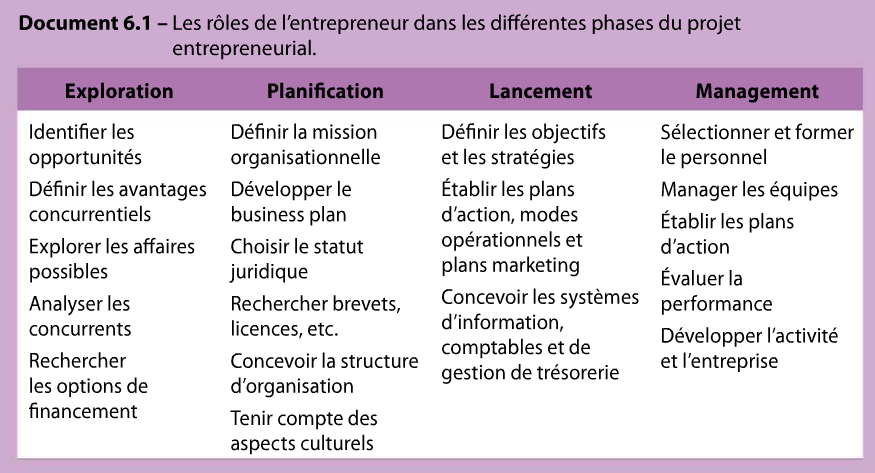
\includegraphics[scale=0.6]{Images/entrepreneuriat}	
	\end{figure}
	\subsection{Nature et objectifs de l'entreprise}
		\point \myul{Fond de roulement} : Argent n\'ecessaire pour lancer l'entreprise et la faire tourner
		\subsubsection{Business Plan}
			\point \myul{Un business plan complet} contient les \'el\'ements suivants :
				\begin{itemize}
				\setlength{\itemsep}{0pt}
			    \setlength{\parskip}{0pt}
			    \setlength{\parsep}{0pt}
				\item \myul{R\'esum\'e op\'erationnel} : \hl{Contient les objectifs et les strat\'egies} de
					l'entreprise, les personnes cl\'es, la nature des activit\'es, des descriptions
					concices des produits et services, une courte explication du cr\'eneau que l'entreprise
					occupera et les avantages concurrentiels.
				\item \myul{Analyse de l'opportunit\'e} : \hl{D\'ecrire le march\'e cibl\'e}, \'evaluer les
					tendances du secteur et \'evaluer les concurrents.
				\item \myul{Analyse contextuelle} : On y d\'ecrit l'\hl{environnement} dans lequel
					l'entreprise vient s'implanter (\'economie, politique, ...)
				\item \myul{La description de l'activit\'e} : Explique comment l'activit\'e sera 
					\hl{organis\'ee}.
					\begin{itemize}
						\setlength{\itemsep}{0pt}
					    \setlength{\parskip}{0pt}
					    \setlength{\parsep}{0pt}
						\item Description pr\'ecise de la mission strat\'egique.
						\item Description de la culture d'entreprise souhait\'ee.
						\item Plans marketing (prix, strat\'egie de vente, garanties, publicit\'es, ...).
						\item Plans de d\'eveloppement de produit (difficult\'es, risques, co\^uts).
						\item Plans op\'erationnels (installations, am\'eliorations, \'equipement, ...).
						\item Organisation des RH (directeurs, composition du CA, ...).
						\item Tableau chronologique d'ensemble d'\'ev\'enements. 
					\end{itemize}
				\item \myul{Les donn\'ees financi\`eres} : Couvre au moins 3 ans, \hl{pr\'evision des 
					b\'en\'efices, des bilans \textit{pro forma}}, le tout avec notes explicatives.
				\item \myul{Documents annexes} : Tableaux, graphiques, photos, ...					
				\end{itemize}\noindent
			\point \myul{Un business plan simplifi\'e} consiste au r\'esum\'e op\'erationnel et de 
				propositions \\\alinea commerciales sur les tenants et aboutissants de l'entreprise.
		\subsubsection{Documents annexes}
			\point \myul{Plan d'affaire} : Document de \hl{synth\`ese} \`a l'attention des parties prenantes 
			    dans lequel \\\alinea est d\'ecrit le business model et les \'etapes et les ressources
			    et n\'ecessaires \\
			\point \myul{Business Model} : Partie du plan d'affaire expliquant \hl{comment l'entreprise 
				g\'en\'erera}\\\alinea de la valeur et sera rentable. Y pr\'evoir l'\'evolution de   
				l'entreprise sur au moins \\\alinea 3 ans, et faire une projection des co\^uts et 
				b\'en\'efices.
		\subsubsection{Organisation du projet}
			\point \myul{Les facteur principaux} du statut juridique sont : la fiscalit\'e, la
				responsabilit\'e \\\alinea l\'egale et la marge de manoeuvre.\\
			\point \myul{La structure} de l'entreprise doit \^etre organique (voir Chap. 7). 
				La structure \\\alinea démarre en étoile et, lorsque le nombre d'employé dépasse 
				le nombre maximum de \\\alinea subordonnés que l'entrepreneur peut avoir, elle se 
				transforme en organigramme fonctionnel.\\
			\point \myul{Recruter} des gens \hl{motiv\'es} et passion\'es et les \myul{maintenir} en offrant
				des \hl{compensations} \\\alinea (psychologiques, formations au choix, reconnaissance des 
				capacit\'es)
	\subsection{Diriger une activit\'e entrepreneuriale}
		\point \myul{Profil entrepreneurial} : \red{Haut niveau d'\'energie, une grande pers\'ev\'erance, 
			beaucoup de \\\alinea ressources, de l'autonomie, et un besoin d'ind\'ependance.}\\
		\point \myul{Personnalit\'e proactive} : \red{Agissement d\'elib\'er\'e pour \hl{influencer son 
			environnement}, \\\alinea chercher des opportunit\'es et chercher \`a s'en servir.}\\
		\point Deux m\'ethodes pour acqu\'erir \myul{la motivation} des employ\'es sont la 
			r\'esponsabilisation \\\alinea et la d\'el\'egation.\\
		\point \myul{Deux r\^oles} de l'entrepreneur : diriger l'entreprise et diriger les \'equipes de
			travail.\\
		\point \myul{Les types d'\'equipes} de travail sont : 
			\begin{itemize}
				\setlength{\itemsep}{0pt}
			    \setlength{\parskip}{0pt}
			    \setlength{\parsep}{0pt}
			    \item \red{Les \'equipes responsabilis\'ees} : capables de planifier et d'ex\'ecuter les 
			    	am\'eliorations de processus.
			    \item \red{Les \'equipes autonomes} : responsables d'un grand nombre d'activit\'es 
			    	manag\'eriales
			    \item \red{Les \'equipes transversales} : personnes venant de diff\'erents services
			    	collaborant ensemble.
			\end{itemize}
	\subsection{Piloter l'activit\'e entrepreneuriale}
		\point \myul{Piloter l'entreprise} d\'epend du contexte de l'entreprise :
			\begin{itemize}
				\setlength{\itemsep}{0pt}
			    \setlength{\parskip}{0pt}
			    \setlength{\parsep}{0pt}
				\item \red{En p\'eriode de croissance} : Respect des grandes fonctions manag\'eriales
					de \hl{planification}, d'\hl{organisation} et de \hl{contr\^ole}.
				\item \red{En ralentissement d'activit\'e} : Pr\'evoir des \hl{plans alternatifs} 
					concernant les finances et la restructuration de l'entreprise.
				\item \red{D\'epart de l'entreprise} : \hl{Capitaliser} sur les ressources et le temps
					investit
					dans l'entreprise, ou dans le cas d'un temps difficile, maximiser ce qu'on peut en 
					retirer.
			\end{itemize}
		\point Il est important que l'entrepreneur \hl{pense \`a sa vie personnelle} : G\'erer ses 
			priorit\'es, \\\alinea savoir d\'el\'eguer, demander conseil, s'occuper directement des conflits,
			d\'evelopper \\\alinea un r\'eseau d'amis et de coll\`egues et \'eviter le stress.
	\subsection{Types de leader et de leadership}
		\point Un entrepreneur peut disposer d'une personnalit\'e et d'un projet propices \`a un
			\hl{leadership} \\\alinea \hl{fort}, mais il est confront\'e \`a des \hl{contraintes
			\'elev\'ees} de ressources et de moyens. 
			\\\alinea \red{Il est important de noter qu'un entrepreneur qui se concentre sur son projet
			en d\'elaissant ses \\\alinea employ\'es se met en danger.\\}
		\point \myul{Intrapreneur} : \red{Collaborateur salari\'e affichant un profil de chef d'entreprise,
			avec un profil \\\alinea autonome et qui essaime via un v\'eritable entrepreneuriat}\\
		\point \myul{Les diff\'erents types d'entrepreneurs} sont les suivants :
			\begin{itemize}
				\setlength{\itemsep}{0pt}
			    \setlength{\parskip}{0pt}
			    \setlength{\parsep}{0pt}
			    \item \red{Le cr\'eateur propri\'etaire} : Visage embl\'ematique, demandeur d'un
			    	investissement maximal de la part de ses employ\'es. Similaire \`a un chef de famille.
			    	Il en arrive parfois \`a ne pas r\'eussir \`a d\'el\'eguer et tout vouloir faire lui-même.
			    \item \red{L'h\'eritier successeur} : Entrepreneur malgr\'e lui, motiv\'e par la pression 
			    	familiale. Souvent compar\'e \`a son pr\'ed\'ecesseur, il faut qu'il puisse s'en
			    	distinguer par un style de leadership original.
			    \item \red{Le manager repreneur} : Double visage : sauveur et usurpateur. Sa popularit\'e
			    	aupr\`es des employ\'es d\'epend de sa r\'eussite \`a sauver/maintenir \`a flot
			    	l'entreprise.
			\end{itemize}\noindent
		\point En conclusion, un entrepreneur doit : revendiquer \hl{l'identit\'e} de l'entreprise, 
			pr\'evoir des \\\alinea \hl{performances coh\'erentes} avec son ambition, cr\'eer une 
			\hl{fiert\'e} chez les employ\'es et avoir une \\\alinea vision \`a \hl{long terme} des choses.
\section{Chapitre 7 : De la structure \`a la culture d'organisation}
	\subsection{Les 6 \'el\'ements d'une structure}
		\subsubsection{La sp\'ecialisation du travail}
			\begin{figure}[H]
				\centering
				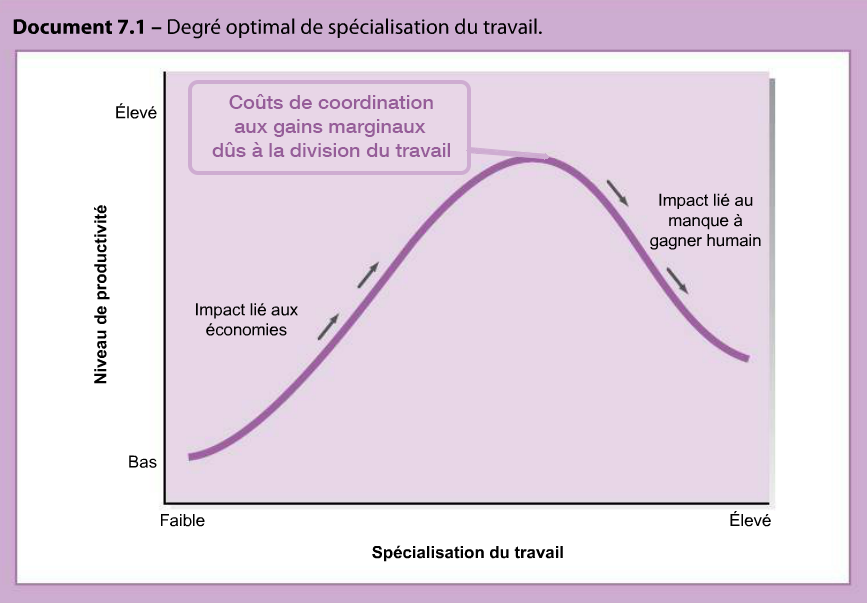
\includegraphics[scale=0.66]{Images/specialisation}			
			\end{figure}
		\subsubsection{La d\'epartementalisation}
			\begin{figure}[H]
				\centering
				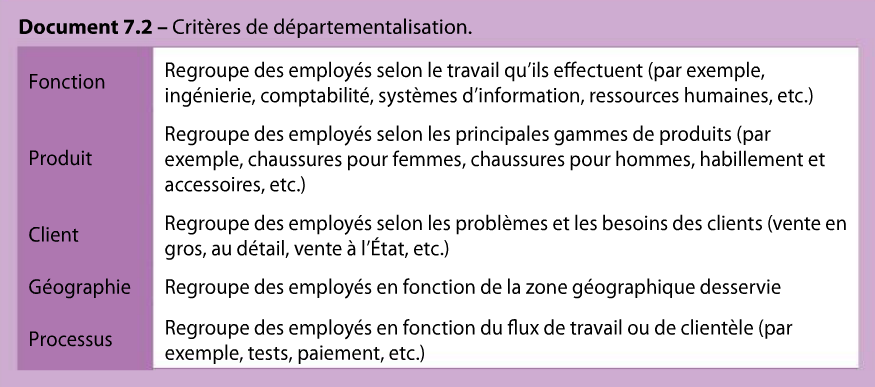
\includegraphics[scale=0.66]{Images/departementalisation}
			\end{figure}
			\point \myul{\hl{D\'epartementalisation par fonction}} : 
				Il y a 3 fonctions que l'on retrouve partout : \\\alinea
				production, commercialisation et administration, et 2 autres qui reviennent \\\alinea
				souvent : RH et R\& D.\\
			\point \myul{\hl{D\'epartementalisation par produit}} ou \myul{Domaine d'Activit\'es Sectorielles}
				(DAS): \\\alinea Pour que ça ait de l'int\'erêt, il faut que les produits puissent être 
				distingu\'es fortement.\\
			\point \myul{\hl{D\'epartementalisation par client}} : Utile lorsque plusieurs cat\'egories bien
				distinctes de clients. \\\alinea Exemple : client de banque souhaitant d\'eposer 100\euro{}
				ou client voulant d\'eposer 1000000\euro{}.\\
			\point \myul{\hl{D\'epartementalisation g\'eographique}} : Utile lorsque la situation de 
				l'entreprise est diff\'erente \\\alinea selon l'endroit. Exemple : Coca challenger en 
				Am\'erique mais leader dans le reste du monde.\\
			\point \myul{\hl{D\'epartementalisation par processus}} : Lorsque les d\'epartements
				repr\'esentent des \'etapes \\\alinea chronologiques  de l'activit\'e de l'entreprise.
				Vieillissant car chaque employ\'e ne se pr\'eoccupe \\\alinea que de sa petite tâche.
			\begin{figure}[H]
				\centering
				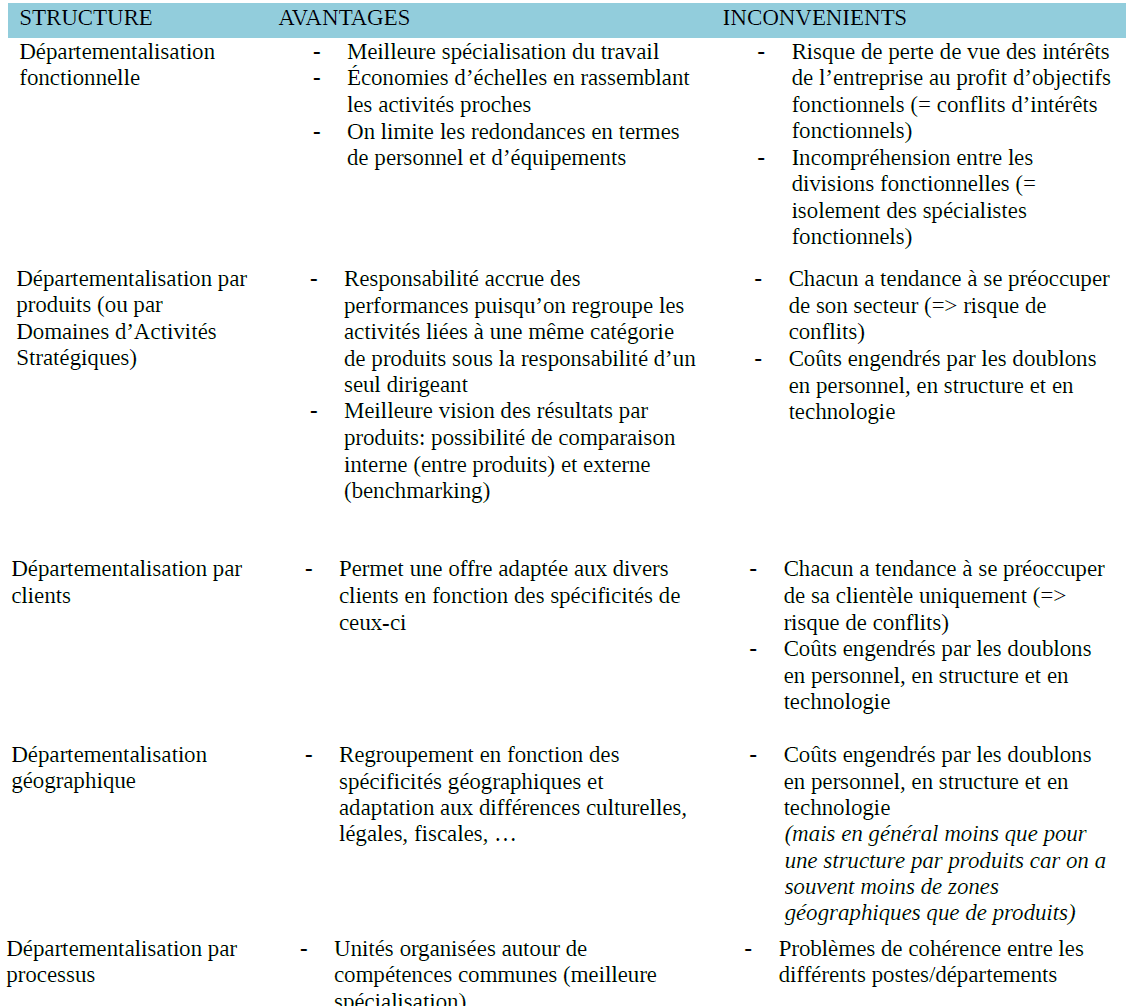
\includegraphics[scale=0.6]{Images/departementalisation1}
			\end{figure}
		\subsubsection{L'autorité et la responsabilité}
			\point \myul{Autorité} : \red{droit inhérent à une \hl{position hi\'erarchique} de donner des 
				ordres et de les \\\alinea voir \^etre ex\'ecut\'es.}\\
			\point \myul{Responsabilit\'e} : \red{\hl{Obligation} de r\'ealiser des tâches assignées.}\\
			\point \myul{Pouvoir} : $A$ a du pouvoir sur $B$ si $A$ peut faire faire quelque chose à $B$
				et que $B$ ne \\\alinea l'aurait pas fait sans l'intervention de $A$.\\
			\point \myul{Autorit\'e hi\'erarchique} : \red{autorité permettant à un supérieur de \hl{diriger 
				le travail} d'un \\\alinea employé}\\
			\point \myul{Autorit\'e fonctionnelle} : \red{autorité revenant à certains postes et devant
				permettre de se \\\alinea  \hl{d\'echarger, d'assister et de conseiller} les détenteurs 
				d'autorité hiérarchique.}\\\alinea Analogie avec l'autorité : Plus on a d'autorité, plus on 
				est proche du centre de pouvoir.
			\begin{figure}[H]
				\centering
				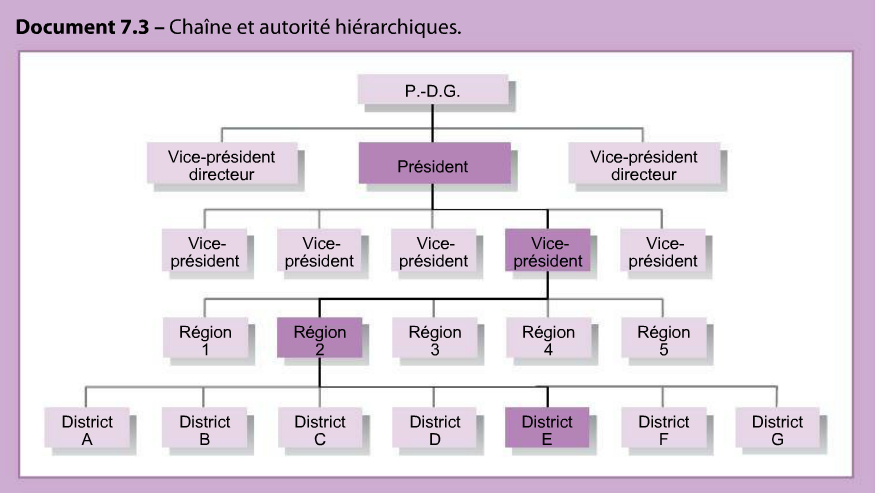
\includegraphics[scale=0.6]{Images/hierarchie}
			\end{figure}				
			\begin{figure}[H]
				\centering
				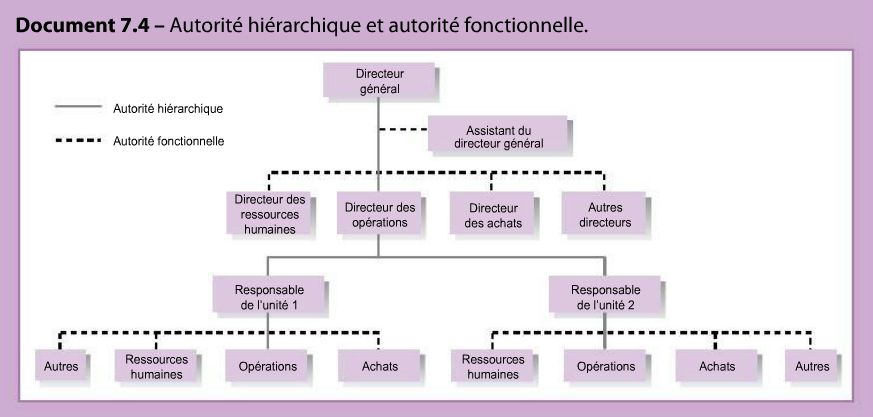
\includegraphics[scale=0.6]{Images/fonction}
			\end{figure}
			\begin{figure}[H]
				\centering
				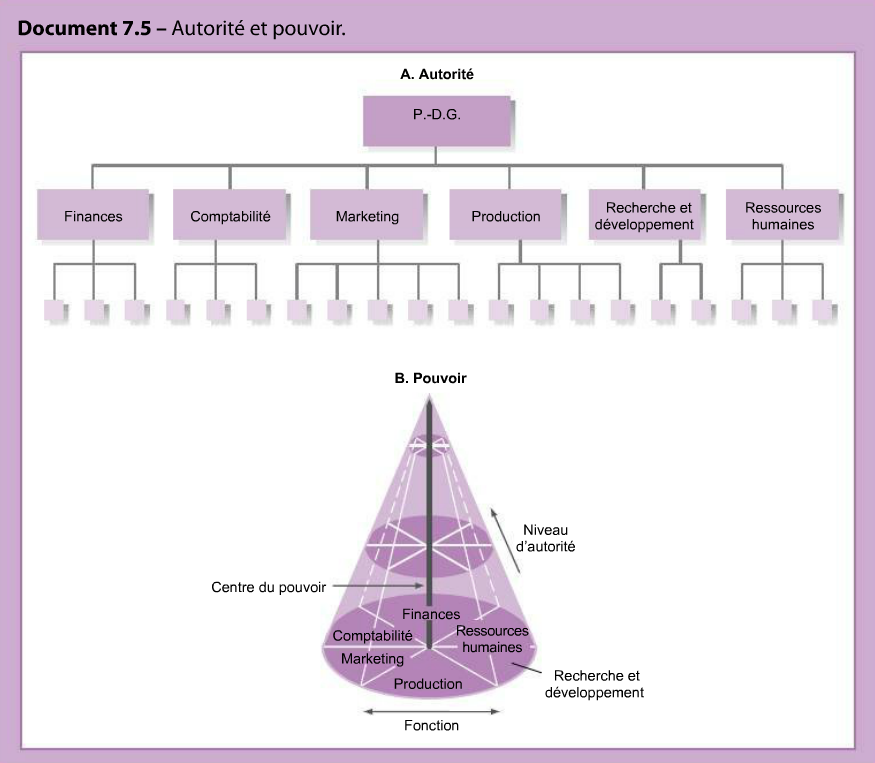
\includegraphics[scale=0.6]{Images/pouvoir}
			\end{figure}\noindent
			\point 5 types de pouvoirs :
				\begin{itemize}
					\setlength{\itemsep}{0pt}
			    	\setlength{\parskip}{0pt}
			    	\setlength{\parsep}{0pt}
			    	\item \myul{Le pouvoir de coercition} : \red{fondé sur la \hl{peur}.} C'est un des
			    		plus simples à mettre en place car c'est une réaction primaire, mais risqué.
			    	\item \myul{Le pouvoir de récompense} : \red{fondé sur la capacité \hl{d'apporter}
			    		ce que d'autres attendent} (dire bonjour, noter les dates d'anniversaire, ...).
			    		Complimenter en public, crucifier en privé.
			    		C'est un des plus simples à mettre en place car c'est une réaction primaire.
			    	\item \myul{Le pouvoir hiérarchique} : \red{fondé sur la \hl{positio}n d'un individu 
			    		dans la hiérarchie.} Ne pas se baser uniquement sur celui-ci, car c'est en 
			    		quelque sort un viol de volonté.
			    	\item \myul{Le pouvoir d'expertise} : \red{fondé sur l'expertise, un \hl{talent 
			    		particulier} ou le savoir de l'individu.} Plus puissant mais nécessite
			    		des capacités.
			    	\item \myul{Le pouvoir de référence} : \red{fondé sur l'identification à une 
			    		personne qui possède les ressources ou les caractéristiques nécessaires,
			    		qui \hl{montre l'exemple}.}Plus puissant mais nécessite des capacités.
				\end{itemize}
		\pagebreak
		\subsubsection{\'Eventail de contrôle}
			\point \red{Nombre d'employés sous sa responsabilité directe qu'un manager peut diriger
				de manière \\\alinea efficace.} (cf. Chap. 13).
		\subsubsection{Centralisation ou décentralisation}
			\point \myul{Centralisation} : \red{mesure dans laquelle les \hl{d\'ecisions} sont prises à des 
				\hl{niveaux \'elev\'es} \\\alinea de l'organisation.}\\
			\point \myul{Décentralisation} : \red{mesure dans laquelle les \hl{niveaux inf\'erieurs}
				de l'organisation \\\alinea contribuent ou sont chargés de la \hl{prise de d\'ecision}.}.\\
			\point Il est important de noter qu'une \hl{structure plate ne veut pas dire d\'ecentralis\'ee}.
				\\\alinea La structure plate indique une faible sophistication, une structure simple, mais
				pas forcément \\\alinea décentralisée. De plus en plus d'organisations responsabilisent
				leurs employés et sont donc\\\alinea décentralisées.
		\subsubsection{Formalisation}
			\point \red{Mesure dans laquelle le travail est standardisé et le comportement des membres de
				l'organisation \\\alinea est déterminé par des règles et des procédures formelles.} Le 
				surcroît de règles peut être \\\alinea contre-productif.
	\subsection{Structure d'organisation}
		\subsubsection{Mécaniste ou organique}
			\point On peut choisir entre une structure organique ou mécaniste selon les critères suivants:
				\begin{itemize}
					\setlength{\itemsep}{0pt}
			    	\setlength{\parskip}{0pt}
			    	\setlength{\parsep}{0pt}
			    	\item La stratégie : Innovation par la différenciation $\rightarrow$ Organique.\\
			    		Stratégie par la minimisation des coûts $\rightarrow$ Mécaniste.
			    	\item La taille : Plus la taille est grande plus il y a de chance que l'entreprise soit 
			    		mécaniste. Si une petite entreprise organique embauche de façon exponentielle,
			    		elle doit pouvoir devenir mécaniste à un certain moment.
			    	\item La technologie : Fabrication spécifique, non routinière $\rightarrow$ Organique.\\
			    		Fabrication routinière $\rightarrow$ Mécaniste.
			    	\item L'environnement : Stable $\rightarrow$ Mécaniste car ne peut pas réagir vite au
			    		changement\\Dynamique $\rightarrow$ Organique.
				\end{itemize}
			\begin{figure}[H]
				\centering
				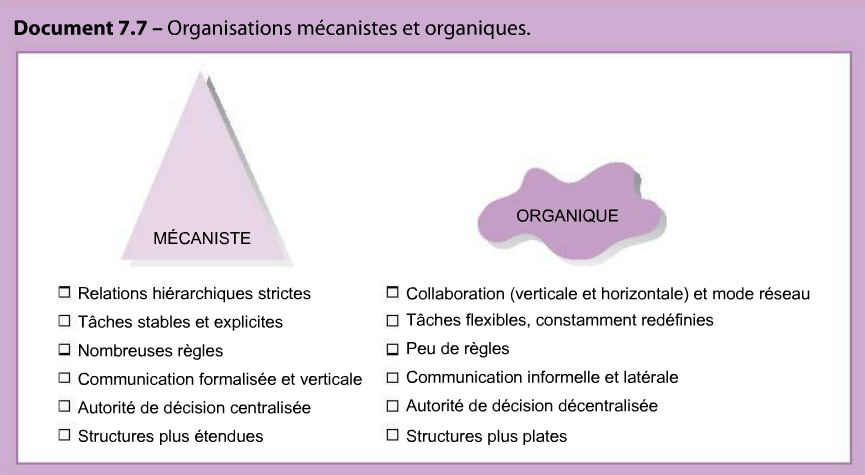
\includegraphics[scale=0.75]{Images/structure}
			\end{figure}
		\subsubsection{Les types de structures classiques}
			\point \myul{Structure plate} ou simple : \hl{D\'epartementalisation faible}, larges 
				éventails de
				subordination \\\alinea une forte centralisation de l'autorité et un faible degrés de 
				formalisation.\\
			\point \myul{Structure par fonction} : Organisations dans lesquelles des \hl{activit\'es
				similaires}	et liées entres \\\alinea elles sont regroupées
			\begin{figure}[H]
				\centering
				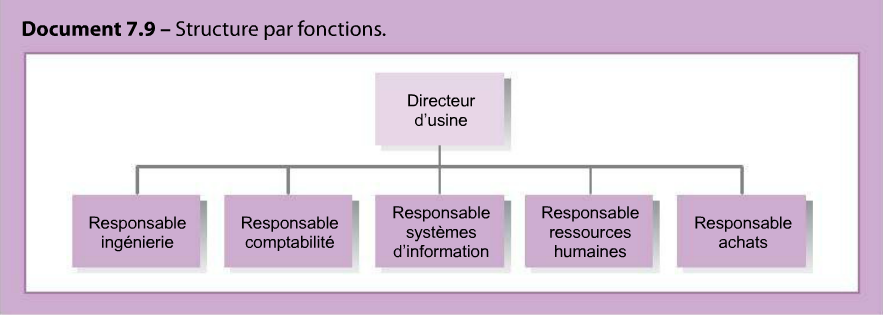
\includegraphics[scale=0.75]{Images/fonctions}
			\end{figure}\noindent
			\begin{figure}[H]
				\centering
				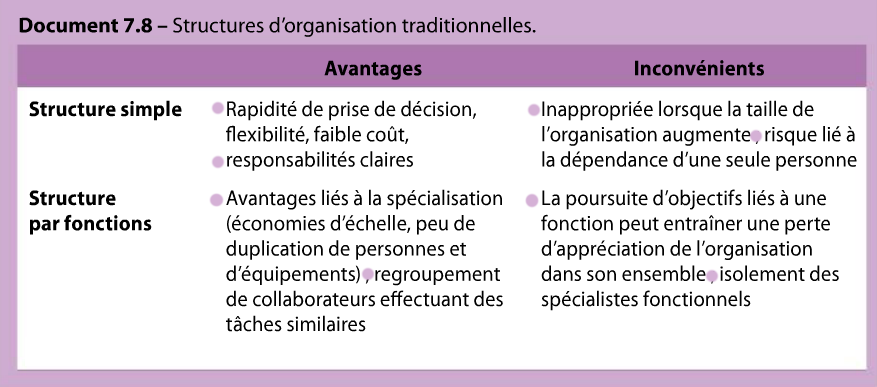
\includegraphics[scale=0.75]{Images/structure2}
			\end{figure}\noindent
		\subsubsection{Les types de structures contemporaines}
			\point \myul{Organisation virtuelle} : \red{Peu de collaborateurs permanents, beaucoup de
				consultants, \\\alinea ce qui permet d'éviter la lourdeur administrative et d'être expert
				dans le projet en cours.}\\
			\point \myul{Organisation en réseau} : \red{A la fois des collaborateurs permanents et des 
				consultants \\\alinea qui sous-traitent les activités en dehors de leur core business.}
			\begin{figure}[H]
				\centering
				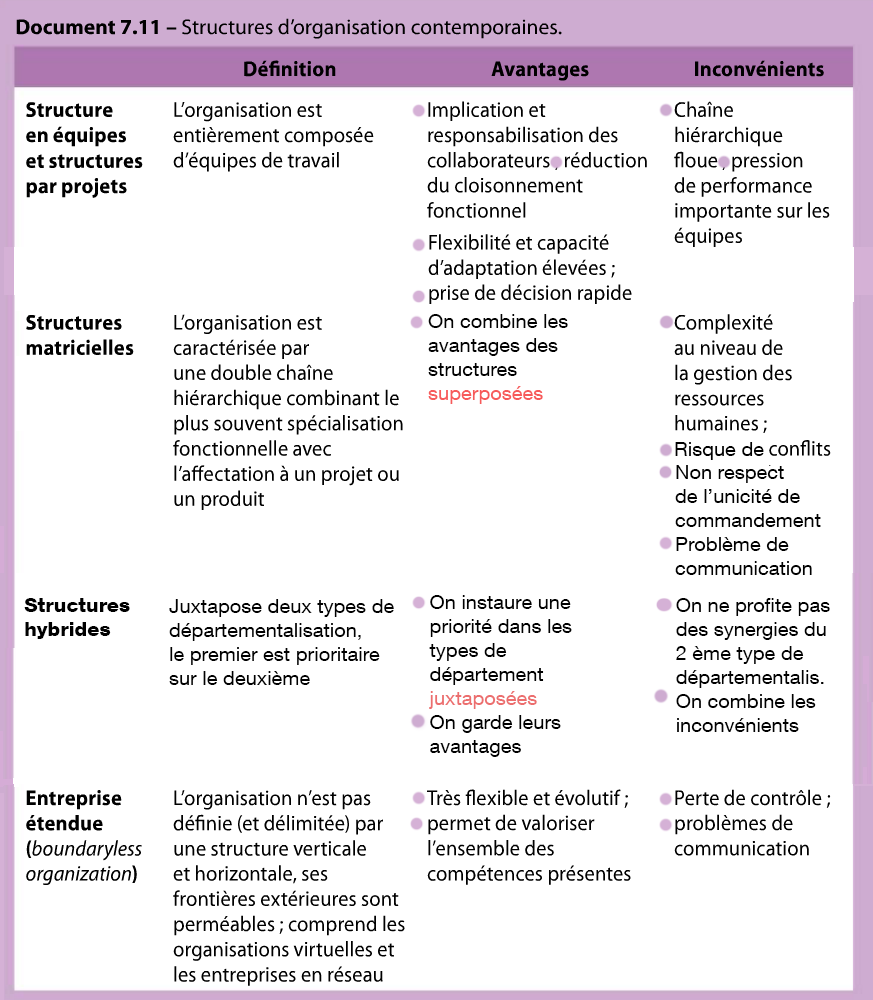
\includegraphics[scale=0.76]{Images/structure1}
			\end{figure}\noindent
			
	\subsection{Mise en place de la structure}
		\subsubsection{Maintien des liens sociaux entre collaborateurs}
			\red{Difficulté de tenir des liens sociaux entre les personnes d'une même équipe répartie
			autour du globe. Solution : Smartphones, videoconférence, réseaux haut débit, vpn, ...}
		\subsubsection{Gestion des organisations mondialisées}
			\red{Faire attention aux différences culturelles entre les différents pays.}
		\subsubsection{Créer une organisation apprenante}
			\begin{figure}[H]
				\centering
				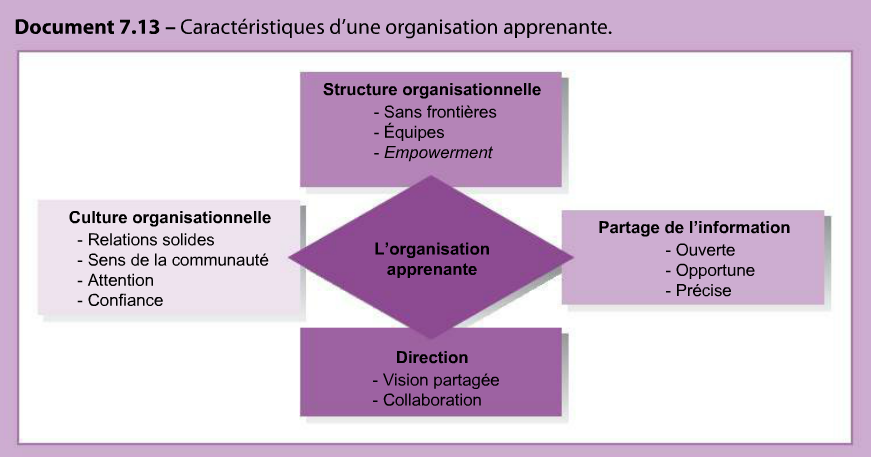
\includegraphics[scale=0.75]{Images/apprenante}
			\end{figure}\noindent
			\point \myul{Boucle simple} : On se donne un objectif auquel on veut parvenir. On compare
				ce qu'on a \\\alinea fait avec cet objectif et on fait en sorte d'en être plus proche la 
				prochaine fois. (Pas suffisant).\\
			\point \myul{\hl{Boucle double}} : Même chose que boucle simple mais à chaque étape on remet 
				en cause la\\\alinea faisabilité de l'objectif.
			\begin{figure}[H]
				\centering
				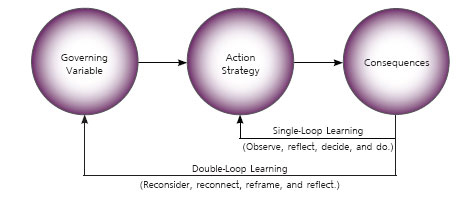
\includegraphics[scale=1]{Images/double_loop}
			\end{figure}\noindent
	\subsection{Méthodes de travail efficientes et efficaces}
		\point \myul{Télétravail} : mode de travail dans lequel les employés travaillent chez eux et sont
			reliées au \\\alinea lieu de travail par le biais d'un \hl{ordinateur}.\\
			\alinea \hl{Avantages} : réduit les coûts d'infrastructure et de carburant et offre plus de 
			 	liberté et de \\\alinea contrôle aux employés sur leur travail.\\
			 \alinea \hl{D\'esavantages} : réduit le sentiment d'appartenance, perte de temps sur les 
			 	jeux/web manque \\\alinea d'interaction sociale, frontières plus floues entre maison et 
			 	travail $\rightarrow$ plus de stress.\\
		\point \myul{Temps flexible} : horaire en 4/5 par exemple $\rightarrow$ réduit les coûts en évitant
			le licenciement\\
		\point \myul{Semaine comprimée} : (4-40) : 4 jours de travail/semaine à 10h/jour par exemple.\\
		\point \myul{Travail partagé} : \hl{Travail} d'un employé \hl{r\'eparti} entre plusieurs personnes.\\
		\point \myul{Travail conjoncturel} : Employer des \hl{consultant}, des CDD, ... au besoin plutôt que 
			des CDI. \\\alinea Implique des difficultés de motivation des employés.		
\pagebreak	
\section{Chapitre 8 : La culture d'organisation}
	\red{Normes, valeurs et croyances, ainsi que principes, traditions et pratiques 
		au sein d'une organisation qui influencent le comportement de ses membres.}
	\subsection{Les 3 niveaux de la culture d'organisation}
		\begin{figure}[H]
			\centering
			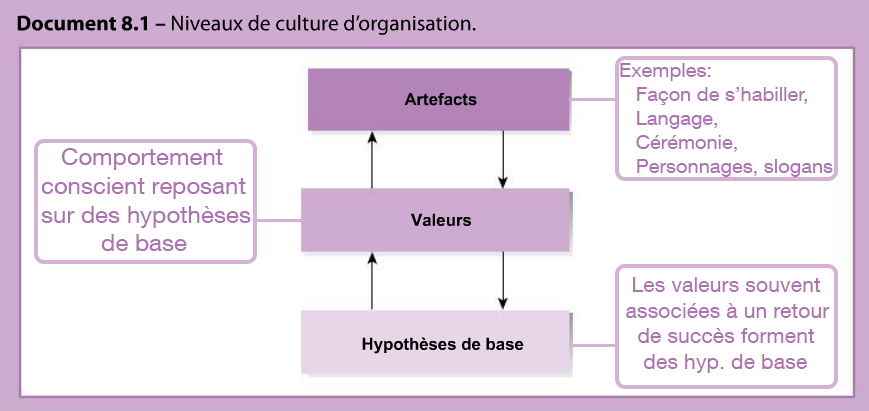
\includegraphics[scale=0.75]{Images/culture}
		\end{figure}\noindent
		\point \myul{Artefacts} : \red{Manifestations \hl{concr\`etes et visibles} de la culture
			d'organisation.}\\
		\point \myul{Valeurs} : \red{Ensemble des normes, qui \hl{guident le comportement}
			\\\alinea des membres de l'organisation.}\\
		\point \myul{Hypothèses de base} : \red{Croyances profondes considérées comme \hl{allant de soi}
			qui\\\alinea constituent le paradigme culturel d'une organisation.}\\
		\point \myul{Cohérence du paradigme culturel} : \red{Il faut que les normes, valeurs et 
			hypothèses de \\\alinea base se \hl{refl\`etent dans les artefacts}.}\\
		\point \myul{Mythes} : \red{Histoires donnant peu d'importance aux faits réels.}\\
		\point \myul{Rites} : \red{Façon de \hl{rassembler} les employés et de marquer le bon et le mauvais
			dans l'organisation.}\\
		\point \myul{Tabou} : \red{Chose tellement inacceptable qu'on ne peut pas en parler.}\\
		\point \myul{Institutions totales} : \red{Organisation dont le membres sont coupés du monde et sont 
			réunis \\\alinea ensemble longtemps.} Il n'y a que dans ces institutions que les membres 
			partagent les mêmes \\\alinea valeurs et hypoth\`eses de base.\\
	\subsection{Comment la culture d'organisation affecte-t-elle une organisation ?}
		\point \red{\myul{Actions sur les employés et leur comportement}}: Les \hl{cultures fortes} 
			(où la plupart des \\\alinea membres partagent la culture) ont plus d'impact que les faibles.\\
			    \alinea \myul{Avantages} d'une culture forte : appartenance à l'organisation, don du 
			    	meilleur de soi-même.\\
			    \alinea \myul{D\'esavantages} d'une culture trop forte : intégration difficile des 
			    	nouveaux employés, \\\alinea \hspace*{0.1cm} déni des informations contraires à leur
			    	culture	et acquisition de société difficile.\\
		\point \red{\myul{Actions sur ce que font les managers}} : La culture d'organisation décrit
			implicitement \\\alinea \hl{ce que peut faire ou non un manager}.
			\begin{figure}[H]
				\centering
				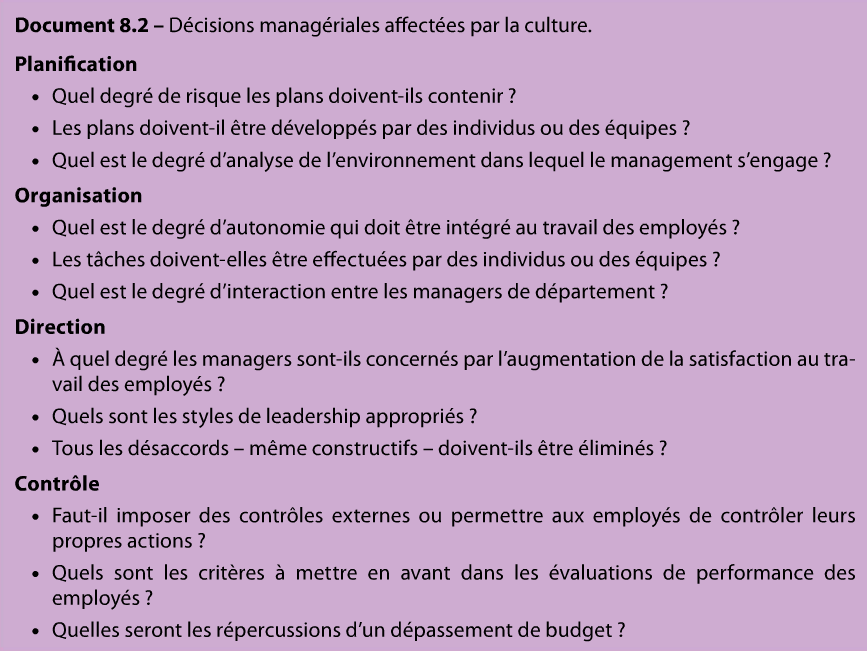
\includegraphics[scale=0.8]{Images/culture_manager}
			\end{figure}
	\pagebreak
	\subsection{Source et direction de la culture d'organisation}
		\point La culture d'organisation vient de \red{(1) les orientations et hypoth\`eses des
			\hl{fondateurs}.
			\\\alinea (2) ce que les premiers employ\'es (et les autres) tirent de leurs \hl{exp\'eriences}.}
			\\\alinea Elle est transmise par les r\'ecits, les rituels, les symboles mat\'eriels et
				le langage.\\
		\point \myul{Récits} : \red{\hl{Personnes/\'ev\'enements} importants.} Crée une image forte des 
			objectifs.\\
		\point \myul{Rituels} : \red{S\'equence d'\hl{actions} r\'ep\'et\'ees}. Exprimentent et renforcent les 
			valeurs et \\\alinea les objectifs de l'organisation.\\
		\point \myul{Symboles mat\'eriels} : \red{Les artefacts qui transpirent les valeurs et objectifs
			de l'organisation.}\\
		\point \myul{Langage} :\red{Jargon/appellations propres à l'entreprise.}
	\subsection{Analyser et manager la culture}
		\point Il ne faut pas conclure du paradigme culturel trop vite. On peut l'analyser selon 7 critères:
		\begin{figure}[H]
			\centering
			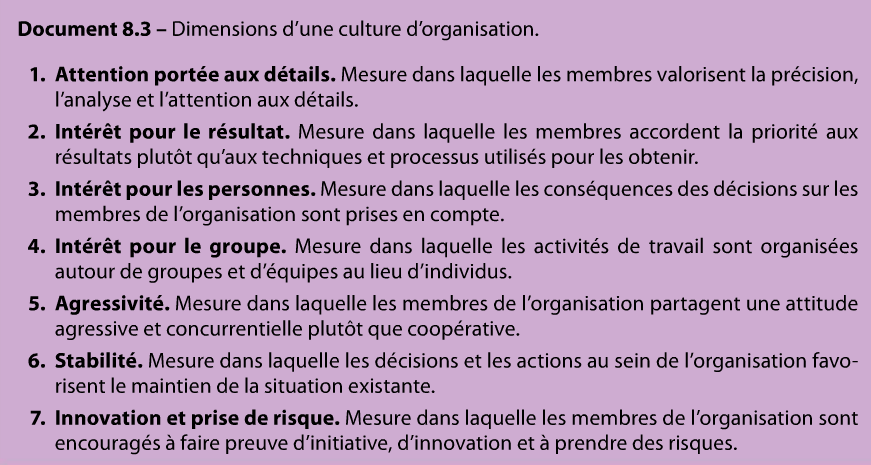
\includegraphics[scale=0.75]{Images/culture_analyse}
		\end{figure}\noindent
		\point On ne peut pas modifier brusquement la culture. Il faut viser le long terme, 
			\\\alinea en modifiant les artefacts par exemple. L'arrivée de nouvelles personnes de culture
			\\\alinea différente l'affecte aussi.
	\pagebreak
	\subsubsection{Cultures nationales}	
		\point \myul{L'\'etude de Hofstede} est un peu dépassée à cause des différences politiques depuis 
			sa mise en place.
		\begin{figure}[H]
			\centering
			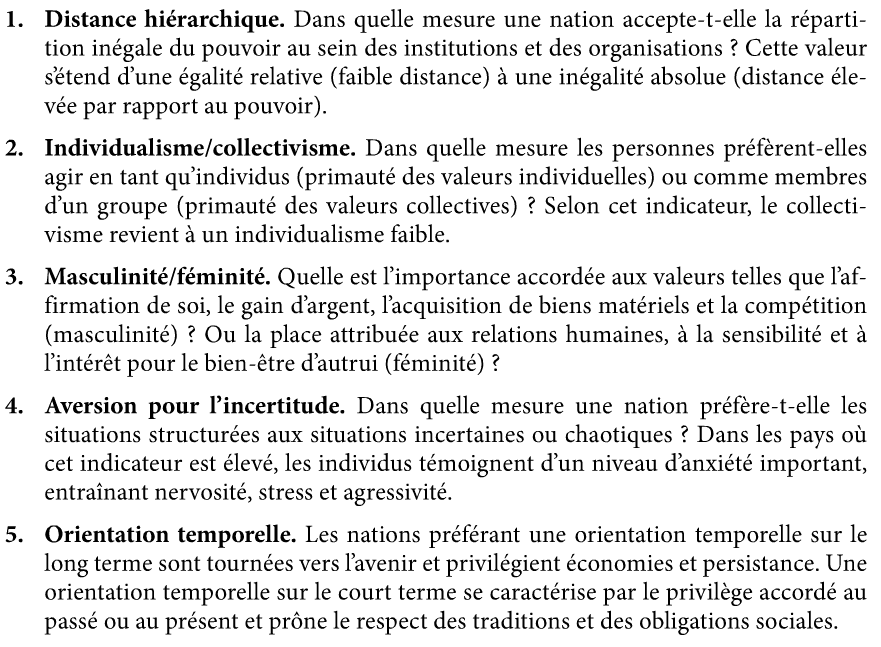
\includegraphics[scale=0.75]{Images/hofstede}
		\end{figure}
		\pagebreak
		\point \myul{L'étude GLOBE} est plus récente et présente de nouveaux critères.
		\begin{figure}[H]
			\centering
			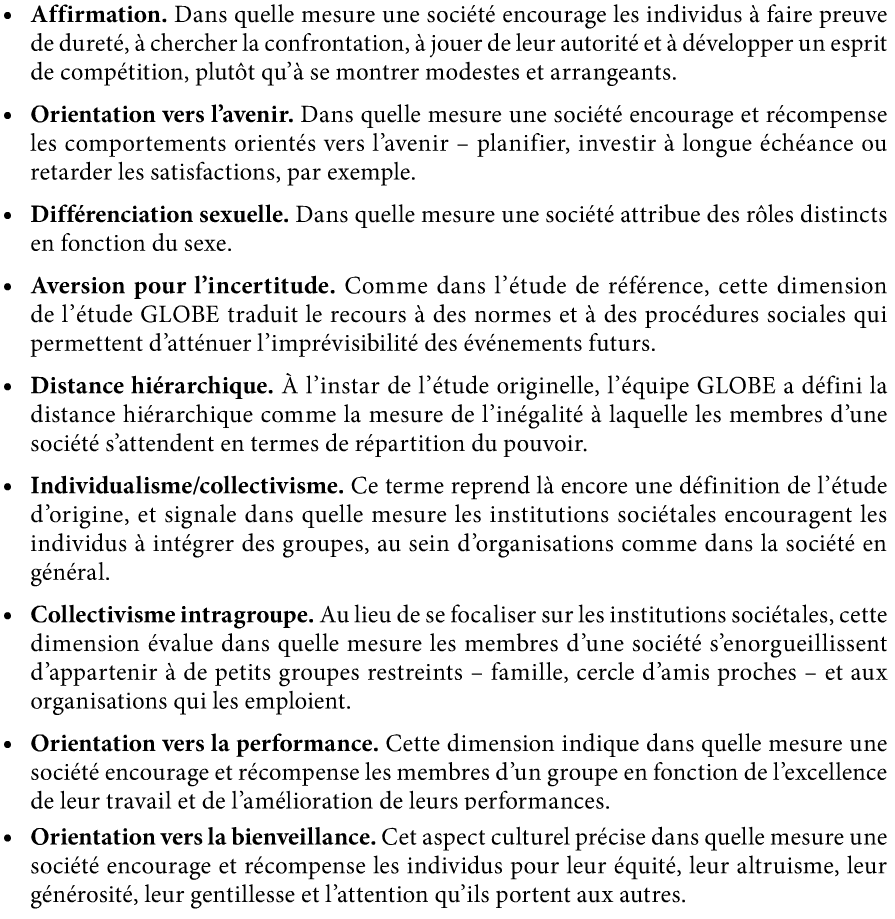
\includegraphics[scale=0.75]{Images/globe}
		\end{figure}
\pagebreak
\section{Chapitre 9 : Le changement et l'innovation}
	\subsection{Qu'est-ce que le changement ?}
		\point \myul{Changement organisationnel} : \red{Modification portant sur la structure, 
			sur la \\\alinea technologie ou sur le personnel d'une organisation.}
		\begin{figure}[H]
			\centering
			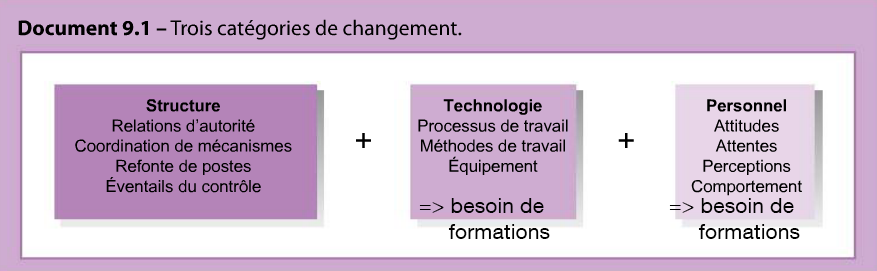
\includegraphics[scale=0.75]{Images/changement}
		\end{figure}\noindent
		\point Il existe des \myul{forces} poussant au changement :
		\begin{figure}[H]
			\centering
			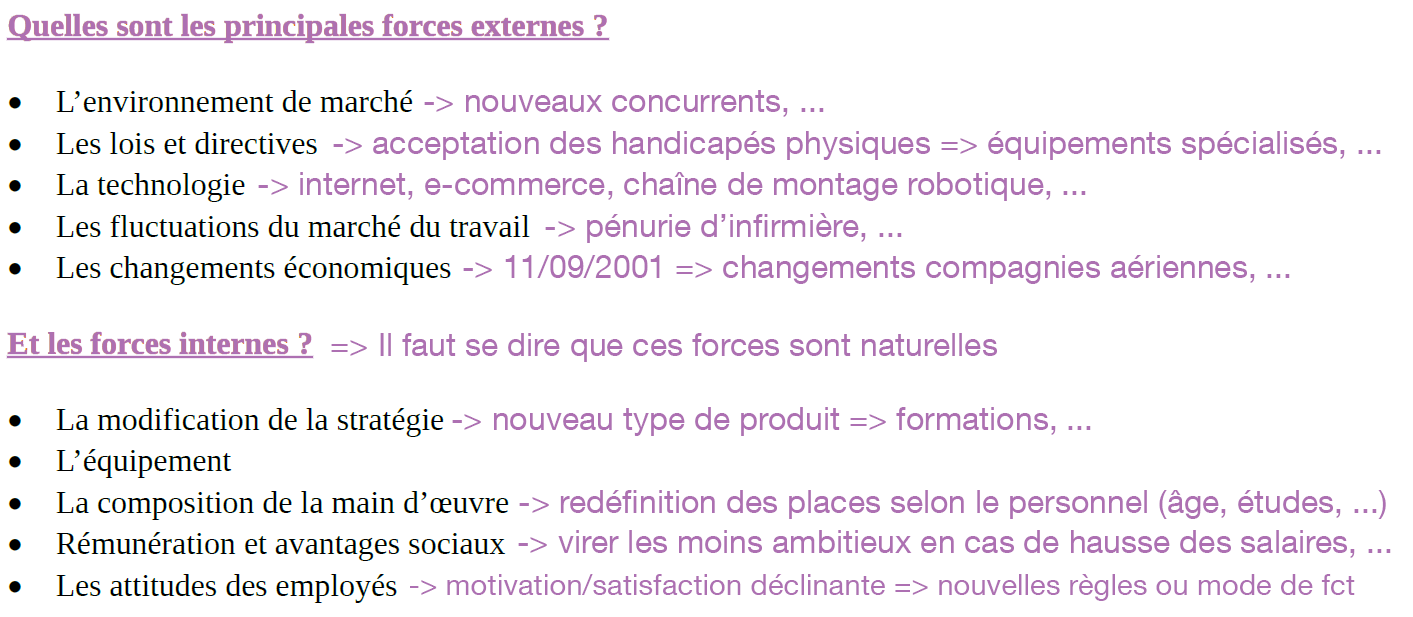
\includegraphics[scale=0.45]{Images/forces}
		\end{figure}\noindent
		\point \myul{Agent de changement} : \red{Individu ou groupe qui sert de \hl{d\'eclencheur} et assume
			les \\\alinea \hl{responsabilit\'es} de gestion du processus de changement.}\\
		\point \myul{Changement en eaux tranquilles} : \red{"\hl{Mer d'huile}", la route est connue et une
			"tempête" \\\alinea se produit de façon occasionnelle pendant un court instant.} Très rare
			au vu du monde actuel.\\
		\point \myul{Changement en eaux vives} : \red{"\hl{Descente de rapide}", situation permanente 
			d'incertitude, de \\\alinea perte de repères et d'aléatoire.} Réactivité et flexibilité sont
			donc essentielles.
		\subsubsection{Eaux tranquilles}
			\point \myul{Le modèle de Kurt Lewin} est très efficace, mais très lent. Applicable 
				en cas de \\\alinea contraintes de temps faibles.
			\begin{figure}[H]
				\centering
				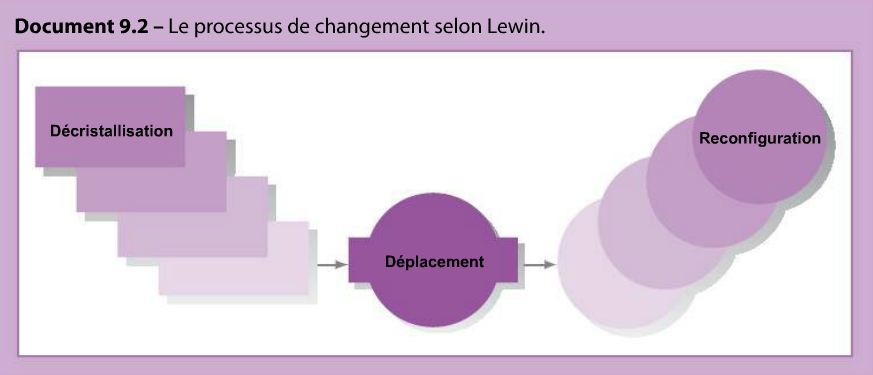
\includegraphics[scale=0.6]{Images/tranquilles}
			\end{figure}\noindent
			\point \myul{Décristallisation} : peut se produire de trois mani\`eres diff\'erentes :
				\begin{itemize}
				 	\setlength{\itemsep}{0pt}
				 	\setlength{\parskip}{0pt}
				 	\setlength{\parsep}{0pt}
				 	\item Les \hl{forces motrices favorables} écartant le comportement du statu quo			
				 		peuvent être \\\hl{intensifi\'ees}.
				 	\item Les \hl{forces antagonistes} empêchant tout éloignement de l'équilibre peuvent
				 		être \hl{r\'eduites}.
				 	\item Mélanger les deux premières. 
				\end{itemize}
			\point \myul{Déplacement} : besoin d'une nouvelle situation d'\hl{\'equilibre} avant de finir le 
				changement.\\
			\point \myul{Reconfiguration} : rupture de l'équilibre et recherche d'un \hl{nouvel \'equilibre} 
				d'après \\\alinea changement.
		\subsubsection{Eaux vives}
			Les techniques ci-dessous fonctionnent \'egalement pour le changement en eaux calmes.
			\point \myul{Développement organisationnel} : \red{Approche du changement planifié basé
				sur les membres \\\alinea de l'organisation et principalement orientée vers les \hl{attitudes
				et les valeurs}.}\\\alinea Débute par un changement de la culture d'organisation.\\
			\point \myul{Enquête de rétroaction} : \red{Méthode permettant d'évaluer les attitudes 
				et les perceptions \\\alinea des employés par rapport aux changements.} 
				\\\alinea Les questions posées portent sur la prise de décision, la direction, l'efficacité
				de la \\\alinea communication, la satisfaction professionnelle, les collègues et 
				le management.\\
			\point \myul{Consultation dynamique} : \red{Recours à des consultants externes qui observent
				les interactions \\\alinea sociales pour voir si le changement n'affecte pas de trop les
				employés.}\\
			\point \myul{Team building} : \red{Activité permettant aux groupes de travail de définir
				des objectifs, \\\alinea d'établir des \hl{relations interpersonnelles positives} et de
				clarifier les rôles \\\alinea et responsabilités de chaque membre.}\\
			\point \myul{Intergroup development} : \red{Sorte d'inter-team building, renforce les liens
				entre \hl{plusieurs} \\\alinea \hl{\'equipes}.}
	\subsection{R\'esistance au changement}
		\myul{4 grandes raisons} motivent la résistance au changement : 
			\vspace*{-0.3cm}\begin{itemize}
				\setlength{\itemsep}{0pt}
				\setlength{\parskip}{0pt}
				\setlength{\parsep}{0pt}
				\item \myul{L'incertitude et la perte des repères} : On efface le connu et on fait 
					place à l'\hl{ambigu\"it\'e} et l'incertitude.
				\item \myul{Les routines} : Le besoin de routines est affecté par le changement de celles-ci.
				\item \myul{La peur d'une perte au niveau personnel} : La peur de perdre les acquis, 
					qui ont été parfois le fruit d'un investissement intense.
				\item \myul{Le sentiment que l'évolution n'est pas ce qu'il y a de mieux pour l'organisation}
					: On pense que le changement va causer une perte de productivité ou de qualité.
			\end{itemize}
		\vspace*{-0.3cm}
		\begin{figure}[H]
			\centering
			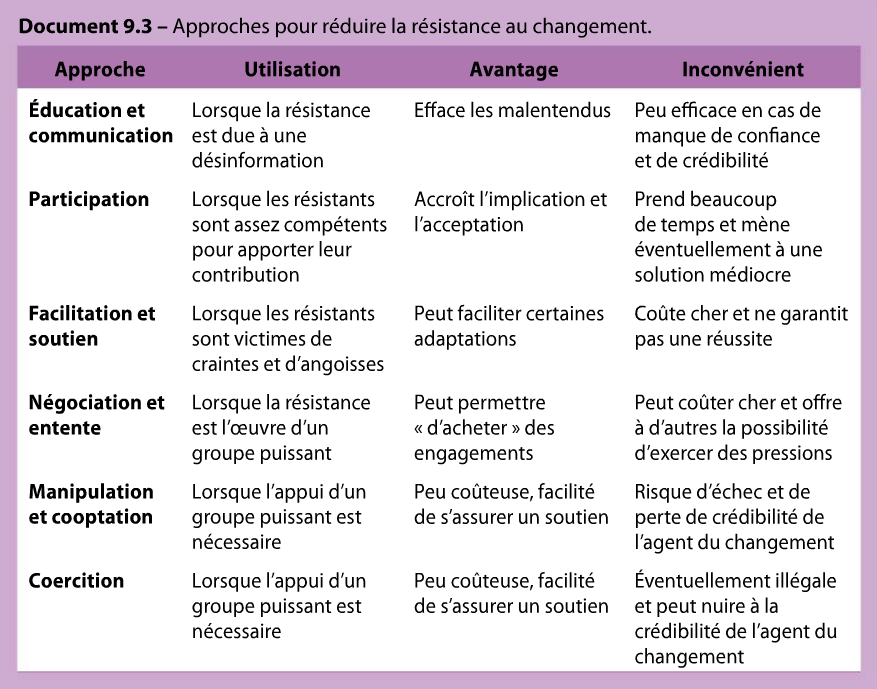
\includegraphics[scale=0.6]{Images/resistance}
		\end{figure}\noindent
	\subsection{Comment les collaborateurs réagissent-ils au changement?}
		\point \myul{Stress} : \red{\hl{Tension} au niveau individuel qui est liée à une pression excessive
			résultant \\\alinea de demandes, de contraintes ou de circonstances exceptionnelles.}
			\\\alinea \myul{Positif} : dépassement de soi quand possibilité de gain.
			\\\alinea \myul{Négatif} : si lié à des contraintes ou des exigences, un risque de perte.
		\begin{figure}[H]
			\centering
			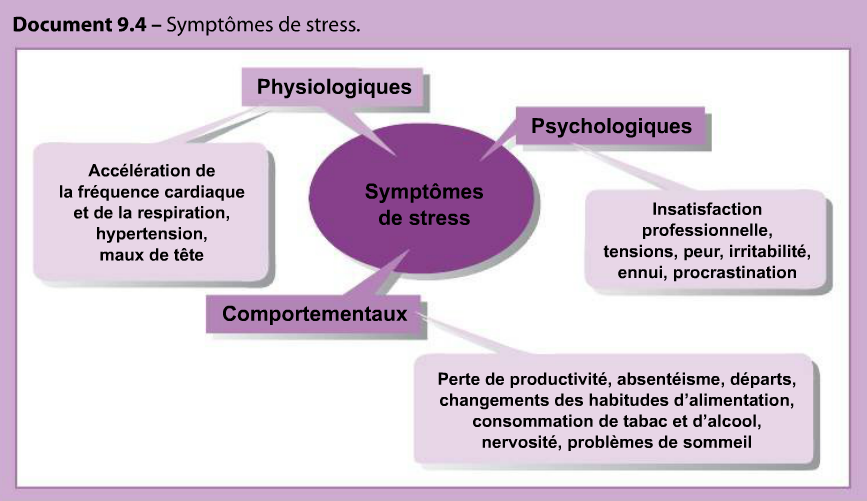
\includegraphics[scale=0.75]{Images/stress}
		\end{figure}\noindent
		\point Le \hl{stress} peut mener les meilleurs éléments à quitter l'organisation; ne reste alors 
			que les mauvais... \\\alinea L'organisation peut proposer un programme d'aide au personnel
			avec des services d'aide\\\alinea physique et psychologique.
		\subsubsection{D'où vient le stress}
			\point \myul{Les obligations de tâches} : \red{Facteurs liés au poste occupé, les 
				\hl{conditions} \\\alinea \hl{de travail} et \hl{l'installation physique}}. ...\\
			\point \myul{Les obligations de rôles} : \red{Liées aux pressions exercées sur une 
				personne \\\alinea en fonction du rôle qu'elle joue dans l'organisation.} 
				\\\alinea Il faut être sûrs que les employés correspondent au poste qui leur est confié
				et \\\alinea éventuellement repenser les tâches afin d'atténuer une éventuelle surcharge.
				\begin{itemize}
					\setlength{\itemsep}{0pt}
					\setlength{\parskip}{0pt}
					\setlength{\parsep}{0pt}
					\item \red{Conflit de rôle} : Attentes professionnelles \hl{difficiles \`a satisfaire}
						parce que contradictoires ou incompatibles. Peut être une demande contraire
						aux valeurs éthiques ou bien devoir choisir entre deux rôles distincts.
					\item \red{Surcharge de rôle} : Avoir \hl{plus de travail} à accomplir que le temps 
						disponible ne le permet.
					\item \red{Ambiguïté de rôle} : Les définitions de \hl{r\^ole sont mal comprises} 
						et causent un sentiment d'incertitude face à ce qu'on attend de l'individu
				\end{itemize}
			\point \myul{Les tensions interpersonnelles} : \red{Pression venant d'\hl{autres employ\'es}.}\\
			\point \myul{La structure organisationnelle} : \red{\hl{Exc\`es de r\`egles} ou 
				de proc\'edures \\\alinea ainsi qu'une \hl{impossibilit\'e} de participer aux 
				d\'ecisions le concernant.} \\\alinea Une solution est de les faire participer à ces
				d\'ecision\\
			\point \myul{Mode de direction} : \red{Certains patrons créent volontairement une culture 
				caractérisée \\\alinea par la création de tensions et la mise en place d'un climat de 
				crainte.}
		\subsubsection{Facteurs personnels de stress}
			\point \myul{Personnalité de type A} : \red{Personnes ayant une \hl{sensation chronique d'urgence}
				un goût \\\alinea excessif pour la compétition sous toutes ses formes et ayant des
				difficultés d'accepter \\\alinea et de profiter du temps libre.} 
				\\\alinea Ceux-ci sont plus enclins au stress.\\
			\point \myul{Personnalité de type B} : \red{Personnes détendues qui \hl{acceptent facilement 
				les changements} \\\alinea et qui ignorent l'urgence et l'impatience.}
	\subsection{Encourager l'innovation au sein de l'organisation}
		\point \myul{Créativité} : \red{Capacité de combiner des idées de façon unique ou inhabituelle}\\
		\point \myul{Innovation} : \red{Correspond au processus de transformation d'une idée 
			créative \\\alinea en produit, service ou méthode.} \\\alinea Elle consiste en 4 \'etapes:
			\vspace*{0.3cm}\begin{itemize}
				\setlength{\itemsep}{0pt}
				\setlength{\parskip}{0pt}
				\setlength{\parsep}{0pt}
				\item \red{La perception} : Façon unique de voir les choses chez chez les personnes
					créatives.
				\item \red{L'incubation} : Réfléchir au problème tout en récoltant une foule d'information.
				\item \red{L'inspiration} : \'Eclair de génie qui permet de trouver la solution.
				\item \red{L'innovation} : Convertir l'inspiration en produit. \'Etape de dévoilement 
					et d'implication d'autres personnes.
			\end{itemize}
		\begin{figure}[H]
			\centering
			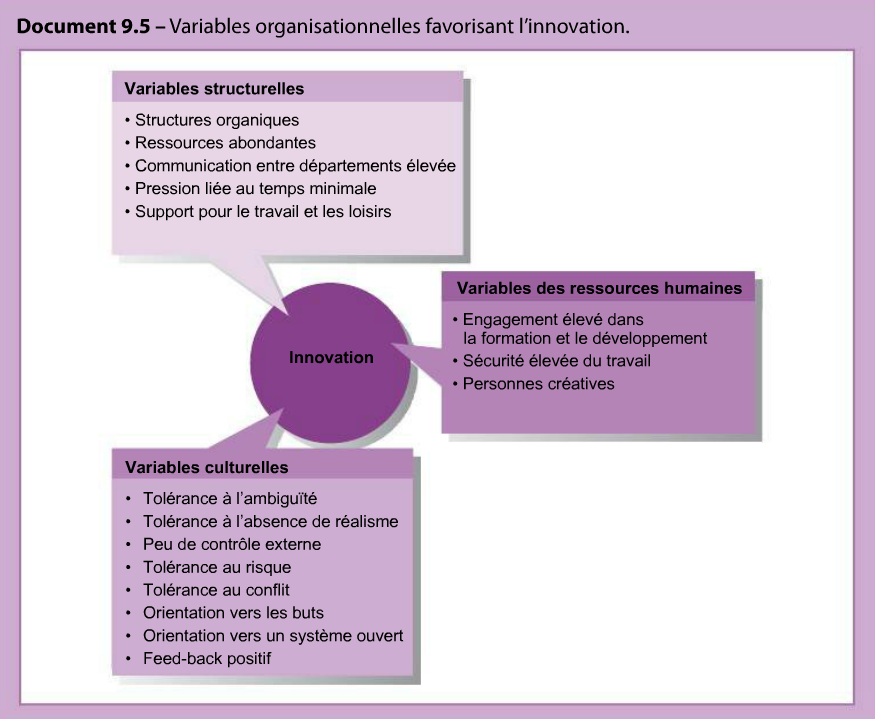
\includegraphics[scale=0.75]{Images/innovation}
		\end{figure}\noindent
	\subsection{Impact de la structure}
		\point Les structures \hl{organiques} sont propices à l'innovation.\\
		\point Les \hl{ressources abondantes} permettent le développement de l'idée.\\
		\point Une \hl{communication fr\'equente} entre les différents services est importante.\\
		\point \'Eviter de trop grosses pressions temporelles.\\
		\point Encourager les employés cr\'eatifs.
	\subsection{Impact de la culture}
		\begin{figure}[H]
			\centering
			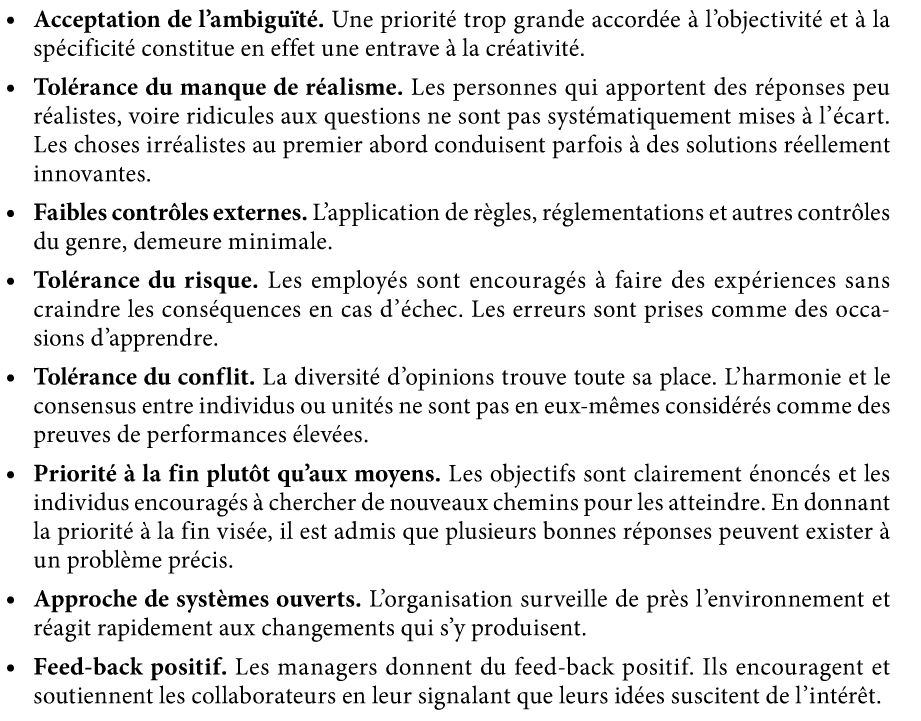
\includegraphics[scale=0.6]{Images/innovation_culture}
		\end{figure}\noindent
\pagebreak
\section{Chapitre 11 : Les groupes et les équipes de travail}
	\point \myul{Groupe} : Deux individus ou plus en interaction et mettant leurs efforts en commun
		pour \\\alinea atteindre des objectifs déterminés.\\
	\point  \myul{Les groupes formels} : Groupes affect\'es \`a des \hl{t\^aches bien d\'etermin\'ees} et
		en lien \\\alinea avec les objectifs organisationnels.
		\begin{figure}[H]
			\centering
			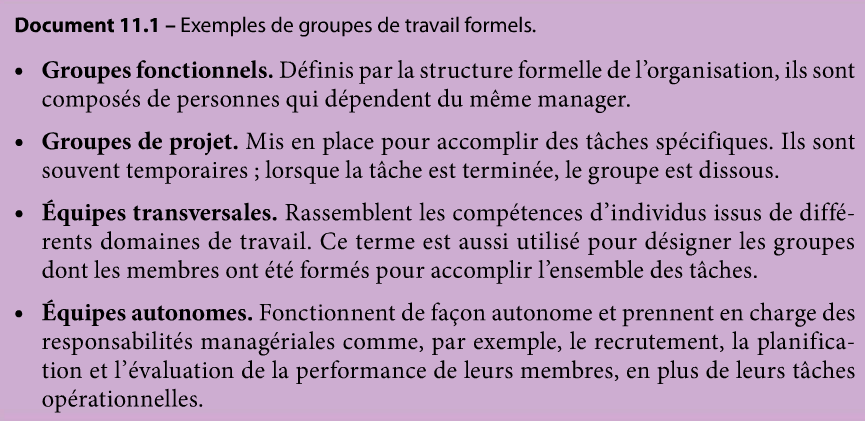
\includegraphics[scale=0.75]{Images/formels}
		\end{figure}\noindent
	\point \myul{Les groupes informels} : Groupes de nature \hl{sociale}. Se base sur l'amitié et les
		affinités.
	\begin{figure}[H]
		\centering
		\includegraphics[scale=0.75]{Images/formation_groupe}
	\end{figure}\noindent
	\point \myul{Rôle} : \red{modèle de \hl{comportement} attendu d'un individu occupant une place spécifique  
		dans \\\alinea l'organisation.}\\
	\point \myul{Normes} : \red{\hl{Standards} ou attentes qui sont acceptés et partagés par les membres 
		d'un groupe.}\\
	\point \myul{Statut} : \red{Position ou rang au sein d'un groupe et conférant un certain prestige.}
		\\\alinea Il est important que les statuts formels soit cohérents (pas de femme de ménage 
		postulant \\\alinea au poste de  PDG).\\
	\point De petits groupes (5-7) seront plus productifs tandis que des grands groupes 
		seront plus \\\alinea innovants. Attention à ne pas arriver à la paresse sociale (les 
		responsabilités sont trop \\\alinea dispersées).\\
	\point \myul{Cohésion de groupe} : \red{Mesure dans laquelle les membres d'un groupe ressentant un
		int\'er\^et \\\alinea mutuel \`a \^etre ensemble et partageant les objectifs du groupe.}
	\begin{figure}[H]
		\centering
		\includegraphics[scale=0.75]{Images/cohesion}
	\end{figure}\noindent
	\point \myul{Groupe de travail} : \red{Plusieurs individus qui décident de s'associer afin 
		d'atteindre \\\alinea des objectifs. Leur performance vaut la somme des contributions
		individuelles. \\\alinea \hl{Aucune synergie n'intervient} pour gonfler le niveau de performance.}
		\\
	\point \myul{\'Equipe de travail} : \red{Groupe dont les membres travaillent de façon 
		intense afin \\\alinea d'atteindre des objectifs partagés. Leur performance se base sur une
		\hl{synergie positive}. \\\alinea La responsabilité est à la fois individuelle et collective.}
	\begin{figure}[H]
		\centering
		\includegraphics[scale=0.7]{Images/groupe_equipe}
	\end{figure}\noindent
	\begin{figure}[H]
		\centering
		\includegraphics[scale=0.7]{Images/performance}
	\end{figure}\noindent
	\point \myul{\'Equipe de résolution de problèmes} : \red{\'Equipe composée de personnes issues
		du m\^eme service \\\alinea apportant des \hl{proposition d'am\'eliorations} suite au 
		"probl\`eme".}\\
	\point \myul{\'Equipe autonome} : \red{\'Equipe fonctionnant \hl{sans manager}. Elle est responsable
		de sa propre \\\alinea gestion et de l'accomplissement de ses objectifs.}\\
	\point \myul{\'Equipe transversale} : \red{\'Equipe composée de personnes issues de \hl{diff\'erents
		services}. \\\alinea Ceci permet de partager les spécialités des différents services pour un
		même but.}\\
	\point \myul{\'Equipe virtuelle} : \red{\'Equipe utilisant uniquement les \hl{technologies 
		modernes} \\\alinea pour communiquer.}
	\begin{figure}[H]
		\centering
		\includegraphics[scale=0.75]{Images/groupe_composition}
	\end{figure}\noindent
	\point On peut former une équipe performante en : (1) sélectionnant des personnes performantes
		et \\\alinea qui s'entendront ensemble (2) formant les membres de l'équipe au travail en équipe
		\\\alinea (3) récompensant les membres méritant et encourager les autres.
	\begin{figure}[H]
		\centering
		\includegraphics[scale=0.75]{Images/multinational}
	\end{figure}\noindent
	\hl{Il faut \'evaluer si les b\'en\'efices li\'es \`a la constitution d'une \'equipe seront 
	sup\'erieurs aux co\^uts ou pas.}
\pagebreak
\section{Chapitre 12 : La motivation}
	\point \myul{Motivation} : \red{\hl{volont\'e} de fournir un effort afin d'atteindre les objectifs 
		fixés par \\\alinea l'entreprise, conditionn\'ee par la capacit\'e de cet effort à satisfaire
		un \hl{besoin personnel}.}
		\\\alinea Dépend de 3 \'el\'ements : l'effort, la direction (les efforts doivent être faits dans
		la direction \\\alinea de l'entreprise) et la pers\'ev\'erance (on veut que les employ\'es
		fournissent des efforts\\\alinea sans baisser les bras). Beaucoup de personnes sont des 
		"zombies" car ils sont démotivés.\\
	\point \myul{L'argent} n'est généralement pas une source de motivation. Pour que ça le soit, il
		faut que: 
		\vspace*{-0.3cm}\begin{itemize}
			\setlength{\itemsep}{0pt}
			\setlength{\parskip}{0pt}
			\setlength{\parsep}{0pt}
			\item L'offre soit significative (passer de 8000 à 8300 est moins motivant que de passer de 
				1500 à 2000).
			\item Qu'il y ait des bonus futurs.
			\item Ce que désire l'employé puisse s'acheter avec de l'argent. (dans le cas
				contraire, on peut par exemple adapter les horaires pour laisser à l'employé plus de 
				temps pour sa passion).
		\end{itemize}
	\subsection{Les théories classiques de motivation}
		\subsubsection{Pyramide des besoins de Maslow}
			Chaque besoin ne s'exprime que si \hl{celui du dessous a \'et\'e combl\'e}.
			\begin{figure}[H]
				\centering
				\includegraphics[scale=0.75]{Images/pyramide}
			\end{figure}\noindent
		\subsubsection{La théorie X et Y de McGregor}
			La théorie Y serait plus valide que la théorie X et qu'il faudrait donc donner des
				responsabilité, de l'autonomie, un travail stimulant et une participation au processus
				de décision permettrait de maximiser l'effort de l'employé. \hl{Rien n'a jamais \'et\'e
				prouv\'e}. Se base sur comment le manager perçoit l'employé.
			\begin{figure}[H]
				\centering
				\includegraphics[scale=0.65]{Images/x_y}
			\end{figure}\noindent
		\subsubsection{La théorie des 2 facteurs d'Herzberg}
			\red{Les deux facteurs selon laquelle il existe des facteurs moteurs permettant d'\hl{accro\^itre 
				la satisfaction} professionnelle et des facteurs d'hygiène permettant de \hl{ne pas
				\^etre insatisfait}.} Se base sur l'influence de l'entreprise.
			\begin{figure}[H]
				\centering
				\includegraphics[scale=0.75]{Images/herzberg2}
			\end{figure}\noindent
			\begin{figure}[H]
				\centering
				\includegraphics[scale=0.75]{Images/herzberg}
			\end{figure}\noindent
		\subsubsection{Théorie des 3 besoins de Mc Clelland}
			Théorie selon laquelle il y a 3 besoins essentiels qui sont des moteurs de motivation.
			\vspace*{-0.3cm}\begin{itemize}
				\setlength{\itemsep}{0pt}
				\setlength{\parskip}{0pt}
				\setlength{\parsep}{0pt}
				\item \myul{Le besoin d'accomplissement} : \red{(ou de réussite). L'envie de \hl{se surpasser}
				et de s'accomplir au delà des normes établies, de se battre pour réussir.} Pour ce besoin 
				on peut donner l'occasion de résoudre des problèmes sous leur responsabilité, leur
				permettre une évaluation rapide et fixer des objectifs pas trop exigeants.
				\item \myul{Le besoin de pouvoir} : \red{Le besoin d'\hl{imposer aux autres} un comportement
				qu'ils n'auraient pas adopté en temps normal.} 
				\item \myul{Le besoin d'affiliation} : \red{Le désir d'établir des \hl{relations
				interpersonnelles} amicales et intimes.}
			\end{itemize}
	\subsection{Les théorie contemporaines de la motivation}
		\subsubsection{La théorie des buts}
			\point \myul{Spécificité} : \red{Des buts spécifiques et ambitieux sont des moteurs de
				motivation.}\\
			\point \myul{Participation} :\red{ La participation des employés à la fixation des objectifs est
				motivante}\\
			\point \myul{Feed-Back} : \red{Lorsqu'un avis est donné sur le résultat, l'employé est motivé à 
				s'améliorer \\\alinea pour se rapprocher du but de performance.} Il y a 3 variables 
				de contingence qui sont \\\alinea susceptibles d'influencer la relation entre le but et 
				la performance:\\
				\begin{itemize}
					\setlength{\itemsep}{0pt}
					\setlength{\parskip}{0pt}
					\setlength{\parsep}{0pt}
					\item \myul{L'engagement face au but} :\red{La théorie des buts fait l'hypothèse qu'un
						individu doit être \hl{psychologiquement engag\'e} vis-\`a-vis du but poursuivi.}
						Ceci peut être amélioré si les buts ont été fixés de façon participative avec
						les collaborateurs.
					\item \myul{Le sentiment personnel d'efficacité} : \red{Croyance qu'a un individu
						dans sa \hl{capacit\'e \`a accomplir} une tâche donnée.} Un faible sentiment
						d'efficacité implique une baisse d'effort dans le but qui paraît insurmontable.
					\item \myul{La culture nationale} : \red{\hl{La th\'eorie des buts peut se voir remise
						en question dans certains pays} qui ne correspondent pas à ces caractéristiques 
						culturelles.}
				\end{itemize}		
			\begin{figure}[H]
					\centering
					\includegraphics[scale=0.75]{Images/buts}
				\end{figure}\noindent
		\subsubsection{Le modèle des caractéristiques de l'emploi (MCE) de Hackman et Oldham}
			Pour cette théorie, tout emploi se définit en fonction de \hl{5 dimensions centrales}:
				\begin{itemize}
					\setlength{\itemsep}{0pt}
					\setlength{\parskip}{0pt}
					\setlength{\parsep}{0pt}
					\item \myul{Variété des tâches} : \red{Le degré de \hl{diversit\'e} du travail.}
					\item \myul{Identité de la tâche} : \red{L'obligation d'accomplir une \hl{t\^ache}
						complète \hl{d\'efinie}.}
					\item \myul{Importance de la tâche} : \red{L'\hl{impact} du travail sur la vie privée et
						la vie professionnelle des autres.}
					\item \myul{Autonomie} : \red{Le degré de \hl{libert\'e et d'ind\'ependance} de l'employé
						quant à l'organisation de son emploi du temps et au choix de ses méthodes de travail.}
					\item \myul{Feed-back} : \red{La possibilité pour l'employé d'avoir un \hl{avis clair et
						rapide} sur l'efficacité de son travail.}
				\end{itemize}
				\begin{figure}[H]
					\centering
					\includegraphics[scale=0.75]{Images/mce}
				\end{figure}\noindent
			\alinea Cette théorie souligne que les \hl{r\'etributions intrins\`eques} s'obtiennent 
				lorsque l'individu
				\hl{apprend} qu'il a \hl{personnellement} accompli de manière satisfaisante une tâche qu'il 
				considère comme \hl{importante}. Celles-ci augmentent \hl{la motivation, la performance
				et le sentiment de satisfaction}, en réduisant dans le même temps le taux d'absentéisme
				au travail. Leurs implications sont modulées par l'intensité du besoin d'accomplissement
				personnel. En effet, l'enrichissement du travail ne fait \hl{aucun effet} chez 
				les individus ayant \hl{un faible besoin d'accom-\\plissement}.\\
			\point \myul{Enrichissement du travail} : \red{Expansion verticale du travail par adjonction
				des \\\alinea responsabilités de planification et d'évaluation.}
			\begin{figure}[H]
				\centering
				\includegraphics[scale=0.75]{Images/mce2}
			\end{figure}\noindent
		\subsubsection{La théorie de l'équité d'Adams}
			\begin{figure}[H]
				\centering
				\includegraphics[scale=0.75]{Images/equite}
			\end{figure}\noindent
			\point \myul{La théorie de l'équité} : \red{Théorie selon laquelle les employés évaluent
				subjectivement \\\alinea ce qu'ils retirent de leur travail (\hl{r\'etributions}, 
				$/!\backslash$ pas uniquement salariales) par rapport
				\\\alinea \`a ce qu'ils y investissent (\hl{contributions}). Ils comparent ensuite ce ratio
				avec celui d'un référent pertinent.} \\
			\point Il y a \hl{3 cat\'egories} auxquelles le référent pertinent peut appartenir :
			\begin{itemize}
				\setlength{\itemsep}{0pt}
				\setlength{\parskip}{0pt}
				\setlength{\parsep}{0pt}
				\item \myul{Autrui} : \red{Les individus possédant un \hl{emploi similaire dans 
					diff\'erentes entreprises}, voire les amis, les voisins et les confrères.}
				\item \myul{Système} : \red{\hl{Politiques et r\`egles salariales} de l'entreprise, ainsi
					qu'à l'administration de ce système. Elle englobe l'ensemble des méthodes de 
					rémunération, implicites comme explicites (barèmes, ...).} On peut comparer des
					personnes qui n'ont pas le même statut. Une tension salariale est le facteur
					entre le salaire le plus bas de l'entreprise et le salaire le plus haut.
				\item \myul{Soi} : \red{Expériences personnelles passées et les \hl{normes personnelles} de
					rétribution/contri-\\bution, ainsi que les obligations familiales.}
			\end{itemize}
		\subsubsection{La théorie des attentes de Vroom}
			\alinea C'est la théorie la plus exhaustive, la plus globale et la mieux établie aujourd'hui. Elle 
			prend comme hypothèse que \hl{l'individu agit dans l'attente d'un r\'esultat donn\'e et en
			fonction de l'int\'er\^et qu'il attribue \`a ce dernier}.\\
			\point \myul{Lien effort-performance} : \red{La probabilité, aux yeux de l'individu, de
				réaliser \\\alinea une performance donnée en fournissant une certaine quantité d'effort.}\\
			\point \myul{Lien de performance-rétribution} : \red{La possibilité, évaluée par l'individu,
				qu'un \\\alinea niveau de performance donné lui permette d'atteindre un résultat donné.}\\
			\point \myul{Intérêt} : \red{L'importance que l'individu accorde au résultat ou à la rétribution
				susceptible \\\alinea de découler de son travail.}
			\begin{figure}[H]
				\centering
				\includegraphics[scale=0.75]{Images/attentes}
			\end{figure}\noindent
			\begin{enumerate}
				\setlength{\itemsep}{0pt}
				\setlength{\parskip}{0pt}
				\setlength{\parsep}{0pt}
				\item \red{Elle souligne l'importance des récompenses et des incitations. Les managers doivent
					s'assurer que les \hl{r\'emun\'erations correspondent aux souhaits des employ\'es}.}
					Chaque individu cherche à maximiser son potentiel de satisfaction pour son 
					intérêt personnel.
				\item \red{Elle incite à \hl{comprendre} pourquoi les employés jugent certaines
					\hl{r\'etributions attrayantes} et d'autres sans intérêt.} Il faut alors offrir les 
					bonnes récompenses aux bonnes personnes.
				\item \red{Il faut que les employés sachent \hl{ce qu'on attend d'eux} et de quelle manière ils
					seront\\ évalués.}
				\item \red{Il ne faut pas s'arrêter à ce qu'on pense mais bien à ce que l'employé 
					\hl{per\c coit}.}
			\end{enumerate}
		\subsubsection{Synthétiser les théories}
			\begin{figure}[H]
				\centering
				\includegraphics[scale=0.75]{Images/motivation}
			\end{figure}\noindent
			\alinea Le chemin idéal est le \hl{chemin du haut} : En faisant son job, il s'auto-accomplit
				et se motive donc intrinsèquement. Le chemin normal, le plus courant, est l'horizontal.\\
	\subsection{Motiver la main d'oeuvre actuelle}
		\subsubsection{Motiver dans un contexte économique difficile}
			\alinea Les employés ont besoin de créativité. Il existe des moyens peu coûteux pour motiver : 
				tenir des réunions de communication, définir des objectifs en commun, souligner 
				l'appartenance à une communauté, formation continue, ...
		\subsubsection{Motiver dans les différentes cultures}
			\alinea Les niveaux de la pyramide de Maslow peuvent être interchangés selon la culture nationale.
				Le critère d'auto-accomplissement et celui d'équité sont peu présents dans certaines cultures.
			\\\alinea Les points communs entre les différentes cultures nationales sont : 
				\begin{enumerate}
					\setlength{\itemsep}{0pt}
					\setlength{\parskip}{0pt}
					\setlength{\parsep}{0pt}
					\item L'importance d'un travail intéressant
					\item L'évolution
					\item La réussite
					\item La responsabilité
				\end{enumerate}
		\subsubsection{Motiver les bas salaires}
			\alinea On peut développer des techniques de valorisation comme l'employé du mois, etc...
			En améliorant les variables du MCE, on peut motiver l'employé en lui donnant l'espoir d'un
			salaire plus élevé.
		\subsubsection{Motiver des techniciens et des professionnels}
			\alinea L'argent n'est plus une motivation pour eux, il faut leur donner des défis au niveau
			de leurs compétences et insister sur le fait que leur contribution est importante. On
			peut aussi les motiver en leur proposant des formations.
		\subsubsection{Motiver des travailleurs temporaires}
			\alinea Ce type d'employé n'est pas facile à motiver. Néanmoins, on peut leur donner 
			l'espoir d'être embauché de façon permanente un jour, ou du moins, leur 
			donner de l'expérience pour qu'ils puissent être engagés ailleurs après leur passage par 
			l'entreprise.
		\subsubsection{Motiver les employés dans les entreprises innovantes}
			\alinea La clé ici est la responsabilisation et l'autonomisation.
\pagebreak
\section{Chapitre 13 : Le leadership}
	\subsection{Les théories classiques du leadership}
		\subsubsection{La théorie des traits de personnalité}
			Pas très précise, plutôt démontée (y compris par le prof) que prouvée...
			\begin{figure}[H]
				\centering
				\includegraphics[scale=0.675]{Images/traits}
			\end{figure}\noindent
		\subsubsection{Les théories comportementale du leadership}
			\paragraph{Kurt Lewin / Université d'Iowa}~\\
				\alinea C'est le style \hl{d\'emocratique} qui obtient les meilleurs résultats 
				de performance et de
				satisfaction. Le non interventionniste n'est pas efficace et l'autocratique est le
				moins satisfaisant.
				\begin{figure}[H]
					\centering
					\includegraphics[scale=0.825]{Images/continuum}
				\end{figure}\noindent
			\paragraph{Université d'Ohio State}~\\
				\alinea Cette théorie a abouti à \hl{deux dimensions} susceptibles de représenter 
				un modèle de leader.
				La théorie indique que le style "high-high", avec une structuration et une considération
				élevée donne les meilleurs résultats. Le \hl{probl\`eme} est que, selon le contexte et 
				la situation,
				trop de structuration donne une accroissement du ressentiment et du taux d'absentéisme et
				que trop de considération implique que le leader ne sera lui-même pas perçu comme performant.
				\\
				\point \myul{La structuration} : \red{Mesure la volonté d'un leader 
					à \hl{d\'efinir} et à \hl{structurer} son rôle et celui de \\\alinea ses employés en vue 
					d'atteindre ses objectifs.}\\
				\point \myul{La considération} : \red{Se rapporte au fait qu'un leader entretient
					des relations de travail \\\alinea caractérisées par l'établissement d'une 
					confiance réciproque et le \hl{respect des id\'ees et des} \\\alinea \hl{sentiments des
					employ\'es}.}
			\paragraph{Université du Michigan}~\\
				Avec un but similaire avec la théorie précédente, elle présente deux dimensions :
				\\\point \myul{Orientation vers l'employé} : \red{Mettre l'accent sur les relations
					interpersonnelles, accorde \\\alinea un int\'er\^et aux \hl{besoins des employ\'es} et 
					accepte leurs différences individuelles.}\\
				\point \myul{Orientation vers la production} : \red{Privilégier l'aspect technique
					ou productif du travail, \\\alinea se préoccupe essentiellement de l'accomplissement
					des tâches assignées au groupe et \\\alinea \hl{consid\`ere ses membres
					comme de simples vecteurs} de cet accomplissement.}
			\paragraph{La grille managériale}~\\
				La grille reprend les dimensions des deux dernières théories et places sous forme de 
				matrice $9\times 9$ différentes positions managériales. La position la plus efficace est
				la $(9, 9)$
				\begin{figure}[H]
					\centering
					\includegraphics[scale=0.75]{Images/grille}
				\end{figure}\noindent
	\subsection{Théories de la contingence}
		\subsubsection{Modèle de Fiedler}
			\alinea Contingence de type leadership / \hl{Situation favorable ou non}. Elle prend d'une part 
			les procédés d'interaction entre le leader et ses subordonnés et le degrés d'influence que lui 
			confère la situation. Les variables pour évaluer la situation seront Les relations
			interpersonnelles, la structuration des tâches ainsi que le pouvoir hiérarchique.
			Ce modèle part du principe que les managers ne peuvent pas s'adapter, et qu'on doit donc 
			changer de manager selon la situation.
			\begin{figure}[H]
				\centering
				\includegraphics[scale=0.75]{Images/fiedler}
			\end{figure}\noindent
		\subsubsection{Le modèle situationnel d'Hersey-Blanchard}
			\alinea Contingence de type leadership / \hl{Maturit\'e du subordonn\'e}. C'est le premier modèle
			situationnel, càd qui considère le leader comme flexible, pouvant s'adapter selon ses employés.
			\\\point \myul{La maturité} : \red{Dans le modèle situationnel, ce terme désigne la
				\hl{comp\'etence} et l'\hl{engagement} d'un subordonné}
			\begin{figure}[H]
				\centering
				\includegraphics[scale=0.75]{Images/hersey}
			\end{figure}\noindent
		\subsubsection{Le modèle de participation du leader de Vroom-Yetton}
			\alinea Contingence de type \hl{Comportement / R\^ole dans le processus de d\'ecision}. 
			Se base sur 12 variables de contingence permettant de \hl{s'adapter \`a la situation}
			Modèle \hl{trop complexe} pour être utilisé de manière régulière.
			\begin{figure}[H]
				\centering
				\includegraphics[scale=0.75]{Images/participation}
			\end{figure}\noindent
		\subsubsection{La théorie de l'objectif-trajectoire de House}
			\alinea Se base sur le modèle de l'université d'Ohio State et sur la théorie des 
			attentes de Vroom. Selon la théorie, le comportement d'un leader demeure acceptable
			tant que ses subordonnés y trouvent une source immédiate ou future de satisfaction.\\
			\alinea \hl{Modification du travail des managers \`a qui il revient d'aider leurs
				subordonn\'es \`a atteindre leurs objectifs, en s'adaptant aux besoins, de chaque 
				employ\'e, en instructions et en soutien.}\\
			\alinea Les leaders peuvent s'adapter en adopter plusieurs styles
				de leadership à la fois:
			\\\point \myul{Le leader directif} : \red{Fait savoir à ses employés ce qu'il attend
				d'eux, \\\alinea \hl{organise la r\'epartition} du travail et donne des 
				\hl{directives sp\'ecifiques}
				en vue \\\alinea de son accomplissement.} Peut s'apparenter à la structuration 
				de l'Ohio.\\
			\point \myul{Le leader bienveillant} : \red{Adopte une attitude \hl{amicale} et se 
				\hl{pr\'eoccupe} \\\alinea \hl{du besoin} de ses employés.} S'apparente à la considération
				de l'Ohio.\\
			\point \myul{Le leader participatif} : \red{Consulte ses employés et \hl{tient compte}
				de leurs \\\alinea \hl{suggestions} avant de prendre une décision.} S'apparente
				au style démocratique \\\alinea participatif de Lewin.\\
			\point \myul{Le leader d'accomplissement} : \red{Fixe des objectifs ambitieux et
				s'attend \`a voir \\\alinea ses employ\'es donner le meilleur d'eux-mêmes.}
			\begin{figure}[H]
				\centering
				\includegraphics[scale=0.75]{Images/objectif_trajectoire}
			\end{figure}\noindent
			\begin{longtable}{|c|c|c|}
				\hline
				\textbf{Style de leadership} & \textbf{Contexte idéal} & \textbf{Contexte à éviter}\\	
				\hline
				\begin{minipage}[t]{2cm}
					\medskip
					\centering
					\textbf{Directif}
					\medskip 
				\end{minipage}
				& 
				\begin{minipage}[t]{6.4cm}
					\medskip
					\begin{itemize}
						\item Tâche ambiguë et stressante
						\item Groupe à tensions et conflits
						\item Collaborateurs pensant que c'est l'environnement 
							qui contrôle ce qui leur arrive
					\end{itemize}
					\medskip
				\end{minipage}
				&
				\begin{minipage}[t]{6.4cm}
					\medskip
					\begin{itemize}
						\item Collaborateurs se considérant comme compétents ou expérimentés
					\end{itemize}
					\medskip
				\end{minipage}
				\\\hline
				%
				%
				\begin{minipage}[t]{2cm}
					\medskip
					\centering
					\textbf{Bienveillant}
					\medskip 
				\end{minipage}
				& 
				\begin{minipage}[t]{6.4cm}
					\medskip
					\begin{itemize}
						\item Tâche très structurée
						\item Relations d'autorité claires
					\end{itemize}
					\medskip
				\end{minipage}
				&\\\hline
				%
				%
				\begin{minipage}[t]{2cm}
					\medskip
					\centering
					\textbf{Participatif}
					\medskip 
				\end{minipage}
				& 
				\begin{minipage}[t]{6.4cm}
					\medskip
					\begin{itemize}
						\item Collaborateurs pensant qu'ils ont le contrôle
							sur ce qui leur arrive
					\end{itemize}
					\medskip
				\end{minipage}
				&
				\\\hline
				%
				%
				\textbf{Accomplissement}
				& 
				\begin{minipage}[t]{6.4cm}
					\medskip
					\begin{itemize}
						\item Tâche structurée de manière ambiguë
					\end{itemize}
					\medskip
				\end{minipage}
				&
				\\\hline
			\end{longtable}
	\subsection{Théories contemporaines du leadership}
		\subsubsection{Interaction leaders-subordonnés (LMX)}
			\alinea Création de groupes préférentiels par le leader. En faire partie est une récompense,
				être en dehors est une punition.
		\subsubsection{Leaders transactionnels ou leaders transformationnels}
			\alinea Les théories précédentes présentaient un type de leader transactionnel. Cette 
			théorie présente un nouveau type, qui n'est pas l'opposé du premier mais qui permet
			d'obtenir des performances plus élevées : le transformationnel.
			\\\point \myul{Leader transactionnel} : \red{Oriente et stimule ses subordonnés
				en \hl{clarifiant les r\^oles et} \\\alinea \hl{les t\^aches} qui leur sont assignées,
				afin de les pousser à atteindre les objectifs fixés.}\\
			\point \myul{Leader transformationnel} : \red{\hl{Incite} ses subordonnés à transcender leurs
				\hl{int\'er\^ets} \\\alinea \hl{personnels} pour le bien de l'entreprise, et poss\`ede
				la capacit\'e d'exercer sur eux une \\\alinea influence durable et profonde.}
		\subsubsection{Leadership charismatique ou visionnaire}
			\paragraph{Charismatique}~\\
				\alinea Un leader charismatique influencent leurs subordonnés en :\\
				(1) leur donnant une vision séduisante du futur \\
				(2) dévoilant ses ambitions et sa confiance en la réussite de ses subordonnés \\
				(3) véhiculant ses valeurs par ses actes et paroles et en devenant un exemple \\
				(4) ne reculant devant aucun sacrifice et affiche une attitude non conformiste.
				\begin{figure}[H]
					\centering
					\includegraphics[scale=0.675]{Images/charismatiques}
				\end{figure}\noindent
			\paragraph{Visionnaire}~\\
				\point \myul{Leader Visionnaire} : \red{Capacité de concevoir et d'énoncer une \hl{vision}
					réaliste, \\\alinea crédible et attractive du futur correspondant à une évolution
					positive de la situation présente.} \\\alinea Le leader doit avoir la capacité 
					d'expliquer sa vision aux autres, pas que sous forme \\\alinea verbale mais aussi 
					par son	comportement. Une vision doit avoir les propriétés
					suivantes : \\
					(1) l'existence d'un potentiel d'inspiration.\\
					(2) des perspectives inspirantes et singulières menant l'organisation vers un avenir
						meilleur.\\
					(3) doit correspondre à la situation actuelle.\\
					(4) doit paraître ambitieuse mais réalisable.\\
		\subsubsection{Le leadership d'équipe}
			\begin{figure}[H]
					\centering
					\includegraphics[scale=0.75]{Images/chef_equipe}
				\end{figure}\noindent
	\subsection{Le leadership aujourd'hui}
		\alinea Le leader aujourd'hui doit pouvoir \hl{responsabiliser} les employés afin de laisser
			un certain contrôle aux personnes sur le terrain. Il peut être nécessaire de se référer
			à l'étude \hl{GLOBE}. Cependant, \hl{le leadership transformationnel} semble être efficace 
			partout. L'intelligence émotionnelle est aussi importante pour le leader d'aujourd'hui.\\
		\point \myul{L'intelligence émotionnelle (IE)} : \red{capacité à percevoir et à gérer des 
			repères et des\\\alinea informations émotionnels.} Elle consiste en 5 points : la 
			conscience de soi, la maîtrise, \\\alinea la motivation, l'empathie et la sociabilité.
	\subsection{La confiance}
		\point \myul{La confiance} : \red{Sentiment de fiabilité envers l'intégrité, le caractère et 
			l'aptitude d'un leader.}
		\begin{figure}[H]
			\centering
			\includegraphics[scale=0.75]{Images/confiance}
		\end{figure}\noindent
		\begin{figure}[H]
			\centering
			\includegraphics[scale=0.75]{Images/construire_confiance}
		\end{figure}\noindent
\pagebreak
\section{Chapitre 15 : les bases du contrôle}
	\point \myul{Le contrôle} : \red{Suivi des activités visant à garantir leur conformité 
		aux \\\alinea préconisations de départ et à corriger tout écart trop important.}
		\\\alinea Il est important principalement dans 3 domaines : la planification, 
		la \\\alinea responsabilisation et la protection de l'entreprise.
	\subsection{Le processus de contrôle}
		\begin{figure}[H]
			\centering
			\includegraphics[scale=0.75]{Images/controle}
		\end{figure}\noindent
		\point Il y a 4 méthodes principales de contrôle : 
			\begin{itemize}
				\setlength{\itemsep}{0pt}
				\setlength{\parskip}{0pt}
				\setlength{\parsep}{0pt}
				\item L'observation personnelle : l'\hl{avantage} est de pouvoir capter les ressentis sur 
					le terrain. L'\hl{inconv\'enient} est que c'est une information subjective.\\
					\myul{Le management baladeur} : \red{Concept décrivant les activités d'un manager 
					qui s'invite sur le lieu de travail et dialogue directement avec les employés.}
				\item Les rapports statistiques : l'\hl{avantage} est de démontrer les liens de 
					causalité. L'\hl{inconv\'enient} est que c'est lent et que ça ignore d'autres 
					facteurs importants.
				\item Les comptes rendus oraux : peuvent se recueillir lors de réunions ou des
					conversations privées. Ses \hl{avantages et inconv\'enients} sont analogues à
					ceux de l'observation personnelle.
				\item Les compte rendus écrits : Leur \hl{avantage} est qu'ils sont très faciles
					à classer et à référencer mais leur \hl{inconv\'enient} est que c'est lent à
					obtenir.
			\end{itemize}	
		\point \myul{Marge de variation} : \red{L'\hl{\'ecart acceptable} entre les performances 
			mesurées et	les normes\\\alinea fixées.}
		\begin{figure}[H]
			\centering
			\includegraphics[scale=0.5]{Images/marge}
		\end{figure}\noindent
		\point \myul{L'action managériale} peut prendre 3 formes :
			\vspace*{-0.3cm}\begin{itemize}
				\setlength{\itemsep}{0pt}
				\setlength{\parskip}{0pt}
				\setlength{\parsep}{0pt}
				\item Ne rien faire.
				\item Corriger les performances :
					\begin{itemize}
						\setlength{\itemsep}{0pt}
						\setlength{\parskip}{0pt}
						\setlength{\parsep}{0pt}
						\item \myul{Action corrective immédiate} : \red{cherche à traiter les 
							problèmes sur-le-champ et de \hl{r\'etablir} aussitôt un \hl{niveau de performance
							ad\'equat}.}
						\item \myul{Action corrective de fond} : \red{consiste à déterminer de quelle
							manière et pour quelles raisons les performances ont dévié, afin de \hl{supprimer
							la source de cette d\'eviation}.}
					\end{itemize}
				\item Réviser les normes.
			\end{itemize}
	\subsection{Les types de contrôle}
		\begin{figure}[H]
			\centering
			\includegraphics[scale=0.675]{Images/controle2}
		\end{figure}\noindent
		\point \myul{Système d'Information de Gestion (SIG)} : \red{Système qui fournit aux managers,
			de façon \\\alinea régulière les informations dont il a besoin.}\\
		\point On veut souvent se concentrer sur l'aspect financier, mais ce n'est pas suffisant
			car on ne \\\alinea se baserait que sur des données passées. 
			\\\alinea Le Balanced Scorecard permet une approche plus générale.\\
		\point \myul{Balanced Scorecard (tableau de bord plurisectoriel)} : \red{approche 
			\hl{multidimensionnelle} \\\alinea de mesure de la performance d'une organisation sans
			se limiter aux seuls aspects financiers.}
			\begin{itemize}
				\setlength{\itemsep}{0pt}
				\setlength{\parskip}{0pt}
				\setlength{\parsep}{0pt}
				\item La perspective financière : plus qu'une simple comptabilité, on va ici
					\hl{utiliser la compta} pour en tirer des conclusions.
				\item La perspective clientèle : \hl{anticiper} sur les résultats futurs selon le
					\hl{contentement des clients}.
				\item La perspective des processus internes : Savoir \hl{ce qui pose probl\`eme en interne}
					afin de l'améliorer.
				\item La perspective des ressources en termes de personnel : rendre le \hl{personnel
					heureux} afin d'améliorer les performances.
			\end{itemize}
\pagebreak
\section{Chapitre 16 : Management des opérations}
	\point \myul{Management des opérations} : \red{La conception, l'exploitation et le contrôle du
		processus \\\alinea de transformation qui permet de convertir des ressources telles que le 
		travail \\\alinea et les matières premières (inputs) en biens et services (output) vendus
		aux consommateurs.} 
		\\\alinea  Il est essentiel étant donné qu'\hl{il s'applique \`a tous les secteurs}, présente une \hl{gestion
		\\\alinea efficace et efficiente de la production} et a un r\^ole strat\'egique en mati\`ere de \hl{comp\'etitivit\'e}.\\
	\point \myul{Processus de transformation} : \red{Le processus par le biais duquel une entreprise
		cr\'ee \\\alinea de la valeur en transformant des ressources en produits finis.}
	\begin{figure}[H]
		\centering
		\includegraphics[scale=0.75]{Images/transformation}
	\end{figure}\noindent
	\point \myul{Entreprise industrielle (ou manufacturi\`ere)} : \red{Entreprise qui produit des
		\hl{bien mat\'eriels}.}\\
	\point \myul{Société de service} : \red{Entreprise qui produit des\hl{ produits immat\'eriels}.}\\
	\point \myul{Productivité} : \red{Rapport entre la production globale des biens et services et les
		ressources \\\alinea n\'ecessaires \`a la production.}\\\alinea
	\subsection{Le management de la chaîne de valeur}
		\point \myul{Valeur} : \red{Concept générique recouvrant les performances, les caractéristiques,
			\\\alinea les \hl{particularit\'es}, ou tout autre aspect d'un bien ou d'un service pour
			lesquels
			le \hl{client} \\\alinea se montre pr\^et \`a \hl{sacrifier certaines de ses ressources}.}\\
		\point \myul{Chaîne de valeur} : \red{Concept décrivant la totalité des activités successives
			qui, \\\alinea \`a chaque \'etapes qui, depuis la manipulation des mati\`eres premi\`eres
			jusqu'au \\\alinea produit fini plac\'e entre les mains de l'utilisateur, \hl{ajoutent de la 
			valeur}. \\\alinea Elle tient compte de tout, des fournisseurs d'un fournisseur jusqu'aux
			clients des clients.}\\
		\point \myul{Gestion de la chaîne logistique} : \red{Processus qui d\'esigne la gestion des 
			installations, \\\alinea des fonctions et des activit\'es qui interviennent dans la 
			production et la livraison \\\alinea d'un produit ou d'un service, du fournisseur au client.
			Elle se concentre sur l'efficience des \\\alinea flux de mati\`eres à destination de 
			l'entreprise et pr\'esente donc une orientation interne. \\\alinea Elle est orient\'ee
			vers l'efficacit\'e et vise \`a offrir le plus de valeur possible aux clients.}\\
		\point \myul{Gestion de la chaîne de valeur} : \red{Processus qui consiste à g\'erer 
			l'encha\^inement \\\alinea des activit\'es et l'information sur les flux de production 
			tout au long de la chaîne \\\alinea de valeur. Cette gestion concerne à la fois les inputs et 
			les outputs, et affiche par cons\'equent \\\alinea une \hl{orientation externe}. Elle est 
			orient\'ee vers l'\hl{efficience}.}\\
		\point On parle d'\myul{amont de la cha\^ine de valeur} quand on regarde du côté 
			matières premières \\\alinea et d'\myul{aval de la cha\^ine de valeur} quand on regarde 
			du côté du produit fini. \\\alinea On peut donc \hl{am\'eliorer} la chaîne de valeur 
			en se \hl{concentrant} en amont et/ou en aval de la \\\alinea cha\^ine.
			L'amélioration de la chaîne de valeur offre plusieurs avantages:
			\begin{itemize}
				\setlength{\itemsep}{0pt}
				\setlength{\parskip}{0pt}
				\setlength{\parsep}{0pt}
				\item L'augmentation des ventes.
				\item La réduction des coûts.
				\item L'augmentation des parts de marché.
				\item La réduction des stocks.
				\item L'amélioration de la qualité.
				\item La réduction des délais de livraisons.
				\item L'amélioration de la logistique.
				\item L'amélioration du service clients.
			\end{itemize}
		\point Les \myul{6 conditions} d'une bonne gestion de la chaîne de valeur sont :
		\begin{itemize}
			\setlength{\itemsep}{0pt}
			\setlength{\parskip}{0pt}
			\setlength{\parsep}{0pt}
			\item \textbf{La coordination et la collaboration} : La \hl{communication} est importante pour 
				que tous les partenaires puissent \hl{identifier ce que le client valorisera}.
			\item \textbf{L'investissement technologique} : De bonnes technologies d'\hl{information} 
				sont essentielles pour la gestion.
			\item \textbf{Les processus organisationnels} : Identifier où est-ce que la valeur est créée
				et quels sont les \hl{services qui n'en cr\'eent pas} afin de les \hl{supprimer}. 
				\\Les 3 méthodes pouvant l'améliorer sont :
				\begin{itemize}
					\setlength{\itemsep}{0pt}
					\setlength{\parskip}{0pt}
					\setlength{\parsep}{0pt}
					\item Une meilleure prévision de la demande.
					\item Une collaboration étroite avec les membres de la chaîne de valeur.
					\item \'Etablir des nouvelles méthodes d'évaluation.
				\end{itemize}
			\item \textbf{L'implication de l'encadrement} : Il est important que les \hl{cadres} soient
				\hl{solides et impliqu\'es}.
			\item \textbf{Les ressources humaines} : Avoir une \hl{bonne main d'oeuvre} implique 3
				conditions:
				\begin{itemize}
					\setlength{\itemsep}{0pt}
					\setlength{\parskip}{0pt}
					\setlength{\parsep}{0pt}
					\item La flexibilité des postes.
					\item Un processus d'embauche efficace.
					\item Un effort de formation continue.
				\end{itemize}
			\item \textbf{La culture de l'entreprise} : Une culture s'appuyant sur la \hl{partage}, 
				la collaboration, l'ouverture, la \hl{flexibilit\'e}, le respect mutuel et la \hl{confiance}.
		\end{itemize}
		\begin{figure}[H]
			\centering
			\includegraphics[scale=0.8]{Images/chaine_valeur}
		\end{figure}\noindent
		\point \myul{Les principaux obstacles à la gestion de la chaîne de valeur:}
			\begin{figure}[H]
			 	\centering
			 	\includegraphics[scale=0.75]{Images/obstacles}
			 \end{figure}\noindent 
	\subsection{La chaîne de valeur d'aujourd'hui}
		\point \myul{La technologie et l'e-fabrication} : Technologies permettant une \hl{gestion du stock}
			en direct, \\\alinea avec des \hl{syst\`emes d'alertes} en temps réel en cas de problème. \\
		\point \myul{L'inventaire Just In Time} : cf. Chapitre 3, stock de matières premières 
			juste \\\alinea suffisant pour assurer la production du moment. => \hl{pas d'argent qui dort}.\\
		\point \myul{Faire de la qualité} : Il faut se fixer des objectifs d'amélioration tout en
			ciblant \\\alinea quels aspects améliorer. Le tout en \hl{contr\^olant} régulièrement la qualité
			produite par rapport à la qualité attendue.
			\begin{itemize}
				\setlength{\itemsep}{0pt}
				\setlength{\parskip}{0pt}
				\setlength{\parsep}{0pt}
				\item ISO 9000 : Certification de qualité pour l'entreprise; indispensable pour 
					l'international.
				\item Six Sigma ($6\sigma$) : Norme visant à ne pas dépasser 3 à 4 défauts par 
					million d'unité ou de procédures.
			\end{itemize}
	\subsection{La gestion de projet}
		\point \myul{Diagramme de Gantt} : \red{Outil de \hl{planification} qui met en regard, sous la
			forme d'un \\\alinea histogramme, les \hl{deadlines} prévues d'une série de tâches 
			et leur \hl{\'etat d'avancement} effectif.}\\
		\point \myul{Diagramme de charge} : \red{Diagramme de Gantt modifié utilisant une liste 
			d'individus ou \\\alinea de ressources.}\\
		\point \myul{Analyse PERT} : \red{Organigramme décrivant les \hl{activit\'es successives}
			nécessaires
			\`a l'accomplissement \\\alinea d'un projet, et pr\'ecisant la \hl{dur\'ee et le co\^ut}
			de chacune d'entre elles.} \\\alinea L'analyse comporte les étapes suivantes :
			\begin{enumerate}
				\setlength{\itemsep}{0pt}
				\setlength{\parskip}{0pt}
				\setlength{\parsep}{0pt}
				\item Identifier les \hl{activit\'es significatives} aboutissant à une étape du projet.
				\item \'Etablir l'\hl{ordre} dans lequel ces étapes doivent apparaître.
				\item \'Etablir les liens de dépendance entre les étapes.
				\item \'Estimer le temps nécessaire à chaque activité.
					\begin{itemize}
						\setlength{\itemsep}{0pt}
						\setlength{\parskip}{0pt}
						\setlength{\parsep}{0pt}
						\item $d_{opt}$ : la durée optimiste
						\item $d_{vrai}$ : la durée vraisemblable
						\item $d_{pes}$ : la durée pessimiste
						\item $d_{pro}$ : la durée probable $= \frac{d_{opt} + 4\cdot d_{vrai} + d{pes}}{6}$
					\end{itemize}
				\item D\'eterminer les dates de début et de fin de chaque étape, le chemin critique 
					(chemin n'admettant pas de retard) et la marge libre (\'ecart de dur\'ee entre
					le chemin critique et tous les autres). 
			\end{enumerate}
		\begin{figure}[H]
			\centering
			\includegraphics[scale=0.75]{Images/gantt}
		\end{figure}\noindent
		\begin{figure}[H]
			\centering
			\includegraphics[scale=0.75]{Images/charge}
		\end{figure}\noindent
		\begin{figure}[H]
			\centering
			\includegraphics[scale=0.75]{Images/pert}
		\end{figure}\noindent
\end{document}























